% Chapter Template

\chapter{Pre-processing Scheme for Fluorescence Microscopy Images} % Main chapter title

\label{chap:Chapter4} % Change X to a consecutive number; for referencing this chapter elsewhere, use \ref{ChapterX}

%\textcolor{red}{There are many factors that degrade the quality of images. The knock-on effect is sub-optimal segmentation results. List the problems and show some images of them. What techniques exist to curb these negative effects? Although it is very common for preprocessing to be done before any further analysis, lack of a scheme. Where do we take this up from (after PSF deconvolution). Why is it non-trivial to design criteria for an ideal image to segment? What do we plan to accomplish in this section?}

%Fluorescence microscopy has become an indispensable tool \citep{Matula2012} in myriad of scientific disciplines such as chemistry, biology, neurobiology and medicine to name a few. It gives scientists visual access to physiological processes and other cellular and sub-cellular activities.
%Fluorescence microscopy coupled with the tremendous technological advancement of image acquisition has lead to an explosion of raw image data such that the sheer volume of images acquired presents too much of a burden on manual analysis \citep{Matula2012}.
%Consequently, there is a need for highly accurate automated analysis.
%In such image analysis, image segmentation has established itself as a key process in identifying and extracting objects of interest which can thereafter be used in higher level image analysis.
%The ever increasing demand on image segmentation is to extract the objects of interest with greater accuracy in a shorter time.

Often enough, the poor results of a segmentation are not because the segmentation method is not tuned properly, or flawed in some way, it is because the image quality is extremely poor which renders acuurate object extraction virtually impossible. 
The fluorescence image acquisition process is ridden with image degradation factors at almost every step.
Yet still, the ever-increasing demand on image segmentation is to extract the objects of interest with greater accuracy in a shorter time.
%There are many factors that degrade the quality of fluorescence images and these can result in sub-optimal segmentations.
%affect the accuracy of the segmentation.
%These factors have been studied independently to a great deal and have been successfully applied to real-world data.
Some of these issues are poor contrast, photo-bleaching, not black enough background, non-fluorescing samples, improper excitation, etc.

Literature is rich with techniques that are able to, a high degree, negate the effect of these factors \cite{Lysaker2004,Wang2008,Zhou2013}. Given the frequency of occurrence of these problems in fluorescence images, it is surprising that there is lack of definition of a scheme prior to segmentation that prepares an image such that accurate segmentation can be achieved.

The task of defining a set of criteria an image has to meet for reliable segmentation results is not a trivial one.
However, segmentation algorithms are desgined to work with certain image charateristics and we can design pre-processing schemes that enhance these characteristics such that  we would have a "better" image to segment. Enhancement of the original image can facilitate higher level analysis e.g. contrast enhancement.
%segmentation qualities. The criteria of this scheme is
In this chapter, we aim to design a hybrid algorithm that builds on highly efficient algorithms to produce better results. A typically fluorescence image segmentation scheme is shown in \Cref{fig:wholescheme}.
In this scheme, a proxy image is generated. This image has the enhanced characteristics required for accurate segmentation. In the next step, segmentation is performed on the proxy image which yields a segmentation mask. The segmentation mask oftens contains speckle and other faux segmetnation areas which are then removed in the clean-up stage.
Thereafter, depending on the next level of image analysis, just the final segmentation mask may be all that is required, otherwise, the mask is overlayed on the original image and sent through for high level analysis.

\begin{figure}[!h]
	\centering
	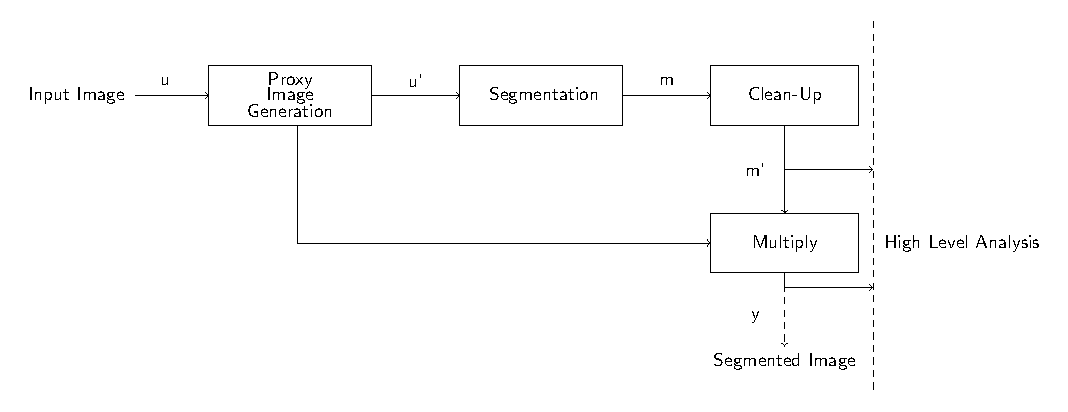
\includegraphics[width=1\columnwidth]{mypreprocess/whole_process}
	\caption{Segmentation Scheme.}
	\label{fig:wholescheme}
\end{figure}

The step that we are concerned with, in this chapter, is the Proxy Image Generation stage. Most segmentation schemes in fluorescence image segmentation would segment on intensity, therefore, a typical pre-processing scheme would emphasise the following main steps:

\begin{enumerate}
	\item Noise reduction
	\item Object data enhancement
	\item Edge completion and enhancement
	\item Reduction of intra-region variance
\end{enumerate}

We base our scheme on this framework. The step through process of the proposed scheme is illustrated in \Cref{fig:flowchartproposedscheme}. For multi-channel images, we first split the image into its channel components and process each on its own. It is at this stage that extraneous channels are discarded. Then noise removal is performed on the remaining channels. The next step involves object data enhancement by suppressing non-object data and amplifying object data. We then combine the channels into a single image and perform intra-region smoothing to reduce intensity variation.

\begin{figure}[!h]
	\centering
	%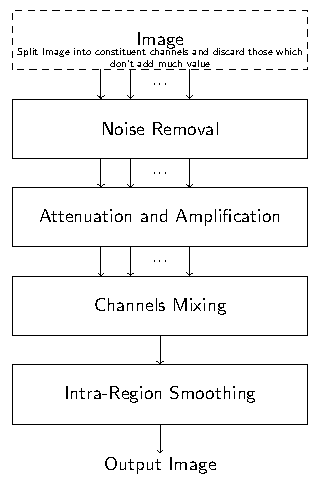
\includegraphics[width=0.25\columnwidth]{mypreprocess/proposed_scheme}
	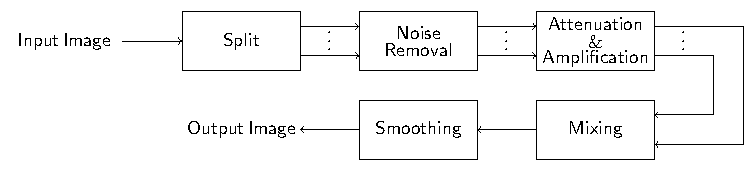
\includegraphics[width=1\columnwidth]{mypreprocess/preprocess_flow}
	\caption{Proxy image generation.}
	\label{fig:flowchartproposedscheme}
\end{figure}

%----------------------------------------------------------------------------------------
%	SECTION 2
%----------------------------------------------------------------------------------------

\section{Pre-processing Scheme}
\label{sec:preprocessscheme}


%----------------------------------------------------------------------------------------
%	SUBSECTION 1
%----------------------------------------------------------------------------------------

\subsection{Denoising}
\label{sec:PoissonDenoising}

\begin{definition}[Removing useless channels]
	Many segmentation algorithms are designed to work on gray scale images. If we have a colour image, it is first converted to gray scale. Previously, each fluorescing sample was captured in a its own grayscale image. The final colour image was composed on a computer. Through the advancements in optical engineering it is now possible for fluorescence images to be obtained in colour, however not all channels add object data to the image.
	%They in fact degrade the image due to the noise in that channel. 
	Often enough, these redundant channels will just be "data-less and noisy", so eliminating this channel will often yield a higher quality image.
	
	For example, a direct conversion of the colour image in \ref{fig:originalgrayscale} to grayscale, shown in \ref{fig:averaginggrayscale}, has lesser brightness, lower contrast and more noise than the grayscale image in \ref{fig:specificgrayscale}, which discarded the data-less blue channel. This is because in a direct grayscale conversion, all channels are averaged to produce the final single-channel image. Hence, the redundant blue channel is suppressing important data.
	
	\begin{figure}[!t]
		\centering
		\subfigure[]
		{
			
			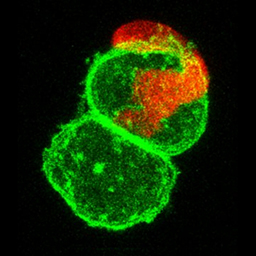
\includegraphics[width=0.31\columnwidth]{mypreprocess/2colr.jpg}
			\label{fig:originalgrayscale}
		}	
		\subfigure[]
		{
			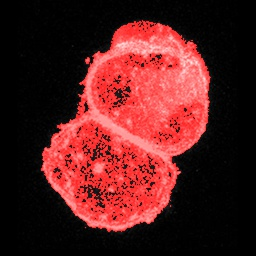
\includegraphics[width=0.31\columnwidth]{cell_database_gray/2gray.jpg}
			\label{fig:averaginggrayscale}
		}
		\subfigure[]
		{
			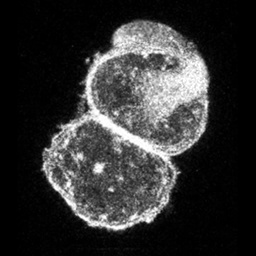
\includegraphics[width=0.31\columnwidth]{mypreprocess/2gr.jpg}
			\label{fig:specificgrayscale}
		}
		\caption{Comparison of grayscale conversions. \textbf{(a)} Original image. \textbf{(b)} Direct grayscale conversion. \textbf{(c)} Grayscale conversion discarding the blue channel.}
		\label{fig:grayscaleconversion}
	\end{figure}
\end{definition}

\begin{definition}[Poisson Noise Reduction]
	In \Cref{sec:ImageProcessing} we mentioned that the primary form of noise in fluorescent images is Poisson noise. It is important to remove as much noise as possible without dampening the boundary information. To this end, we have used the Total-Variation anisotropic denoising (Bregman Split). Although it was developed to remove Gaussian noise, it was shown by Rodriguez \textit{et al.}\citep{Rodriguez2008} that it supersedes other state-of-the-art Poisson noise removal methods, e.g.  wavelets \citep{Timmermann1999}, platelets\citep{Willett2004}, minimum description length \citep{Nowak1999}, while maintaining signal integrity. 
	
	The Poisson distribution, which has equal mean and standard deviation i.e. $\mu = \sigma$, is defined by
	\begin{equation}
	P(n,\mu) = \frac{e^{-\mu}\mu^{n}}{n!}
	\label{eq:poissondist}
	\end{equation}
	
	Let $y = \lbrace y_i:i=1, \cdots, N \rbrace$ and $x = \lbrace x_i:i=1, \cdots, N \rbrace$ be the observed and the true image, respectively. The sample $y_i$ is a Poisson contaminated form of $x_i$. We desire to recover the signal $x$ from the observed signal $y$. From Bayes' Law, we get
	\begin{equation}
	P(x \vert y) = \frac{P(y \vert x)P(x)}{P(y)}
	\label{eq:bayeslaw}
	\end{equation}
	Therefore, we wish to find the maximum of $P(y \vert x)P(x)$. If all samples are affected by Poisson noise we have
	\begin{equation}
	P(y \vert x) = P(y,x) = \frac{e^{-x_i}x_i^{y_i}}{y_i!}
	\label{eq:poissonafect}
	\end{equation}
	Thus the likelihood of observing $y$ given the true image $x$ is given by
	\begin{equation}
	P(y \vert x) = \prod_{i=1}^{N} \frac{e^{-x_i}x_i^{y_i}}{y_i!}
	\label{eq:poissonlikelihood}
	\end{equation}
	
	In anisotropic TV denoising we wish to recover the original image given the noisy image by minimising the constrained problem
	
	\begin{equation}
	\underset{u} {\mathrm{min}} \left| \left| \frac{du}{dx} \right| \right|_1 + \left| \left| \frac{du}{dy} \right| \right|_1 + \frac{\gamma}{2} \left| \left| u-f \right| \right|^2_2
	\label{equ:anisotropic_tv_constrained}
	\end{equation}
	
	where $\gamma > 0$ is the regularisation parameter which affects the balance between noise removal and signal preservation \citep{Getreuer2012}, $u$ is the true image and $f$ is the noisy image. For computational efficiency issues, we actually solve the unconstrained problem
	
	\begin{equation}
	\underset{u, dx, dy} {\mathrm{min}} \left| \left|dx_1 \right| \right|_1 + \left| \left| dy_1 \right| \right|_1 + \frac{\gamma}{2} \left| \left| u-f \right| \right|^2_2 +
	\frac{\lambda}{2} \left| \left| dx-u_x \right| \right|^2_2 + \frac{\lambda}{2} \left| \left| dy-u_y \right| \right|^2_2
	\label{equ:anisotropic_tv_unconstrained}
	\end{equation}
	
	This can be solved using the Bregman Split algorithm \citep{Wei2010}.
	The algorithm runs iteratively until the error, $e = \frac{\vert u'-u \vert}{\vert u \vert}$,  is less than a user-defined tolerance factor, $\epsilon$, where $u'$ is the image obtained after denoising the input image $u$. 
	%We used  $\mu=20$, $\lambda=1$ and $\epsilon=1 \times 10^{-3}$, the original and the denoised channels are shown in Figures \ref{fig:gchannel_1_orig}, \ref{fig:rchannel_1_orig}, \ref{fig:gchannel_1_denoised} and \ref{fig:rchannel_1_denoised}
\end{definition}
%----------------------------------------------------------------------------------------
%	SUBSECTION 2
%----------------------------------------------------------------------------------------

\subsection{Object Data Enhancement}
\label{sec:contrastcorrection}

The fundamental task of binarization of an image is to split up an image into homogenous regions of two gray levels, $l_0$ and $l_1$. All pixels labelled $l_0$ share similar values with regard to the feature under consideration. This also means that there is high dissimilarity with pixels that are labelled $l_1$.
For grayscale images, such as the type we are concerned with, this feature is generally intensity.
For segmentation regarding a specific feature, an ideal image is one where there is no overlap in the feature space between the background and the object, as illustrated in \Cref{fig:featuredataset}. In real images (non-synthetic) this is almost never the case as there is no known feature space or it does not exist.

\begin{figure}[!h]
	\centering
	\subfigure[]
	{
		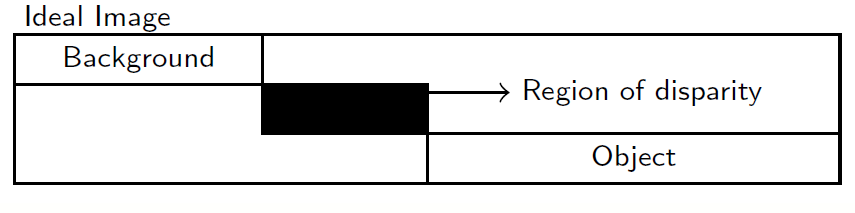
\includegraphics[width=0.48\columnwidth]{mypreprocess/feature_data_set_ideal.png}
		\label{fig:featuredataset_ideal}
	}	
	\subfigure[]
	{
		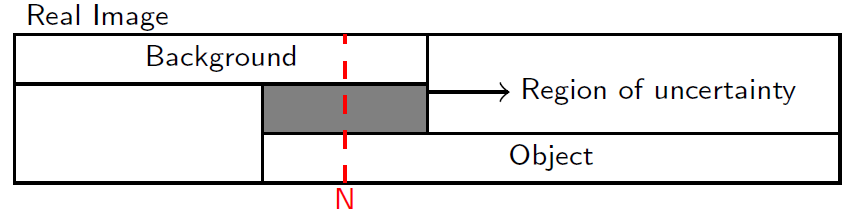
\includegraphics[width=0.48\columnwidth]{mypreprocess/feature_data_set_real.png}
		\label{fig:featuredataset_real}
	}
	\caption{Feature Distribution for ideal and real images. \textbf{(a)} Ideal image. The background and the object occupy distinct non-overlapping partitions of the feature space. The non-overlapping region is called the "Region of Disparity". \textbf{(b)} Real Image. The background and the object partially overlap in the feature space. The overlapping section is called the "Region of Uncertainty".}
	\label{fig:featuredataset}
\end{figure}

Grayscale medical image segmentation (MIS) typically uses intensity as the dominant feature on which the application of the segmentation algorithms is biased. Hence, it is common to precede segmentation by contrast enhancement \citep{Kim2003,Subr2005}. The problem therein lies with the fact that the aim of contrast enhancement is to bring out the details more clearly that are otherwise obscured due to limited dynamic range, non-uniform illumination, etc. In fluorescence image this does not necessarily mean that the contrast enhanced image possesses better "segmentation qualities", in terms of intensity.

In this section, we present a novel mapping function whose aim is to shrink the "region of uncertainty" by non-linearly widening the gap between background pixels and object pixels. This function is composed of two piece-wise sub-functions; one for data attenuation and one for data amplification. We first design the properties the mapping function should have. 

\begin{definition}[Remapping Function Properties]
	We denote the remap function as $\widetilde{x_i} = R(x_i)$, where $\widetilde{x_i}$ is the new value which remaps the input pixel, $x_i$, using the function $R$. The range on which $R$ works is $[0,L]$. For 8-bit gray scale images the highest value is usually $L=255$. 
	Let $N$ be the value that contains the greatest classification uncertainty, as illustrated in \Cref{fig:featuredataset_real}.
	$R$ must have the following properties:
\end{definition}

\begin{enumerate}
	\item{}
	\textit{$R$ must be non-decreasing in the interval $[0, L]$}\\
	This is a trivial criterion arising from the context in which our problem is defined. We specifically focus black background fluorescence images. Consequently, it is not possible for a lower intensity pixel to have a higher probability of belonging to the object compared to a pixel of a higher gray level intensity. 
	
	\item
	\textit{$\widetilde{x_i} = R(x_i=N) = N$}\\
	This value has no bias as to whether it tends more to the background or the object. It is best left unaltered. This is marked in \Cref{fig:remapfunctionspace} as "2".
	
	\item
	\textit{Attenuation: $\widetilde{x_i} < x_i, \, \forall x_i<N$}\\
	$R$ must remap gray-level intensities below $N$, according to $0 \leq \widetilde{x_i} \leq x_i$. This is marked in \Cref{fig:remapfunctionspace} as "3".
	
	\item
	\textit{Amplification: $\widetilde{x_i} > x_i, \, \forall x_i>N$}\\
	$R$ must remap gray-level intensities above $N$, according to $x_i \leq \widetilde{x_i} \leq L$. This is marked in \Cref{fig:remapfunctionspace} as "4".
	
	\item
	\textit{$R'$ must be non-decreasing in the interval $[0,N]$}\\
	Given two pixels, $p_1$ and $p_2$, with values $x_1$ and $x_2$ respectively where $x_1<x_2$. It is more probable for $p_2$ to belong to the object since it has a higher value. Also, pixels with gray levels intensities closer to $0$ do not need to be attenuated as much.
	
	\item
	\textit{$R'$ must be non-increasing in the interval $[N,L]$}\\
	As the pixels values approach $L$, less amplification is needed since the pixels are already more likely to be classified as belonging to the object.
\end{enumerate}

%\begin{figure}[!t]
%	\centering
%	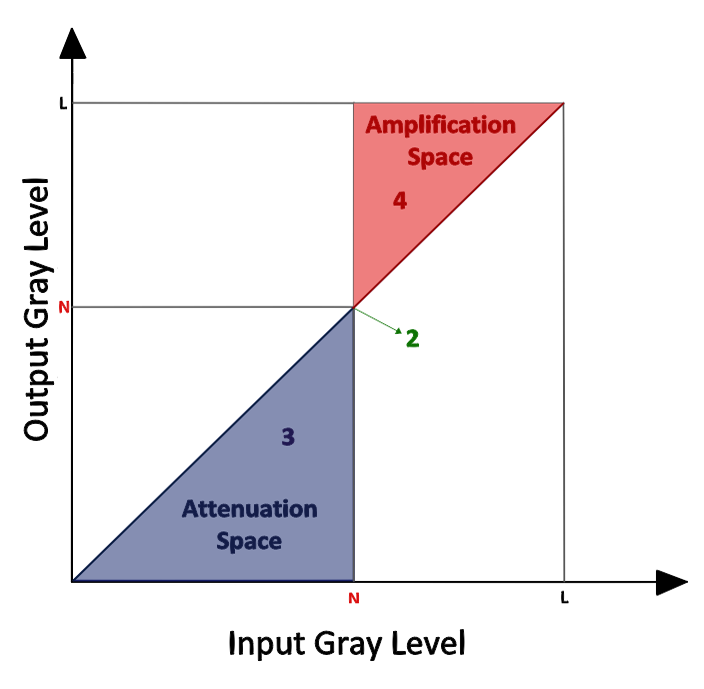
\includegraphics[width=0.45\columnwidth]{mypreprocess/remapfcn_assist.png}
%	\caption{Remapping function space.}
%	\label{fig:remapfunctionspace}
%\end{figure}
%\begin{figure}[!t]
%	\centering
%	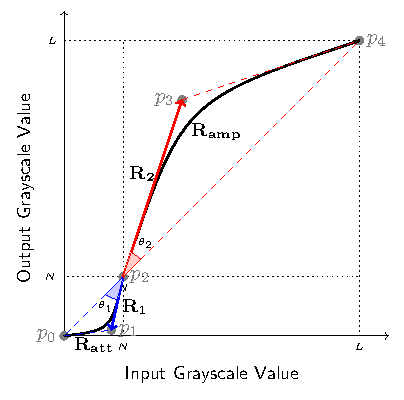
\includegraphics[width=0.45\columnwidth]{remapfcn.pdf}
%	\caption{Plot of remapping function.}
%	\label{fig:remapfcn}
%\end{figure}


\begin{figure}[!t]
	\centering
	\begin{minipage}{.5\textwidth}
		\centering
		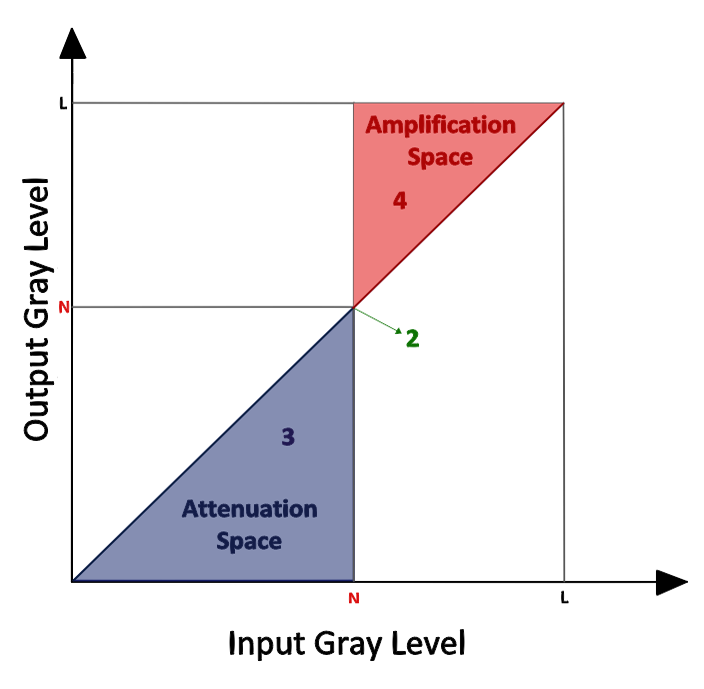
\includegraphics[width=\linewidth]{mypreprocess/remapfcn_assist.png}
		\captionof{figure}{Remapping function space.}
		\label{fig:remapfunctionspace}
	\end{minipage}%
	\begin{minipage}{.5\textwidth}
		\centering
		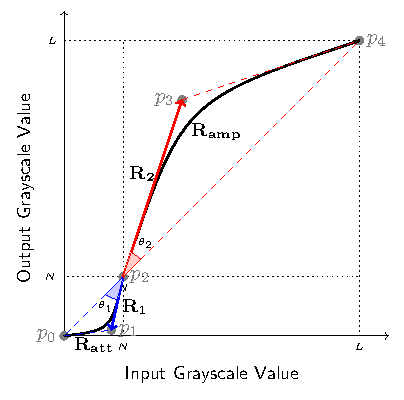
\includegraphics[width=1\linewidth]{remapfcn.pdf}
		\captionof{figure}{Plot of remapping function.}
		\label{fig:remapfcn}
	\end{minipage}
\end{figure}


\begin{definition}[Function Design]
	Given the criteria presented, many functions can be designed. We have decided that one of the better solutions is to make the mapping function a piece-wise quadratic Bezier curve. This is to maintain intuitive tuning of the sub-functions. The two functions are $R_{att}$, for the attenuation section, and $R_{amp}$, for the amplification section as shown in \Cref{fig:remapfcn}.
	
	There are three anchor points the function must pass through. These are $p_0(0,0)$, $p_2(N, N)$ and $p_4(L,L)$. If the curve between $p_0$ and $p_4$ is a straight line, then there is no change between the output and input image since the gradient of the line is equal to $1$. Additional control points are needed to bend the curve.
	There is a particular class of curves whose shapes are useful for our purpose. This places constraints on the position of the control points. Relative to the straight line, $y=x, \, x \in [0,L]$, the amplification curve would be above the relaxed line, $p_{3y} > p_{3x}$, and similarly the attenuation curve would be below the line, $p_{1y} < p_{1x}$. Also, given that the function is to be a one-to-one function, the control point for the attenuation function $p_{1x}<N$; similarly, the control point for the amplification function $p_{3x}>N$.
	
	It is more geometrically intuitive to represent the control points in polar coordinates with the centre at $p_2(N,N)$. Therefore, control point $c$ is represented as $p_c(R_c, \theta_c)$; where $\theta_c \in [0, \frac{\pi}{4}]$ and $R_c \in \mathbb{R}^+$. The angular deviation is the measure off the straight line which is counter-clockwise for the amplification function and clockwise for the attenuation function. The deviation, $\theta_c$, where $c \in {1,2}$, away from the straight line is further implicitly represented as a range $\kappa_c \in [0,1]$ where $\kappa_c=0$ implies $\theta_c = 0$ would mean no deviation, and $\kappa_c = 1$ implies $\theta_c = \frac{\pi}{4}$ would mean maximum deviation.
	As the function approaches the ends of its domain, less attenuation or amplification occurs, which meets criteria 5 and 6.
	
	\begin{figure}[!t]
		\centering
		\subfigure[Amplification function controls points.]
		{
			
			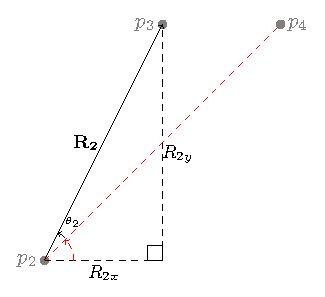
\includegraphics[width=0.48\columnwidth]{attenutation_control_points.pdf}
			\label{fig:ampcontrolpoints}
		}	
		\subfigure[Amplification function curve.]
		{
			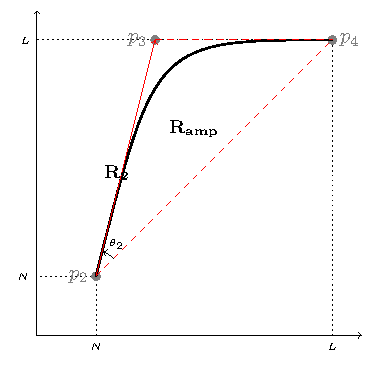
\includegraphics[width=0.48\columnwidth]{attenutation_curve.pdf}
			\label{fig:ampcurve}
		}
		\caption{Amplification function control points and curve.}
		\label{fig:ampcalculation}
	\end{figure}

	The position of the attenuation control point is calculated as
	\begin{equation*}
		{p_1} = \left(
		p_{2x} - R_1\cos[\frac{\pi}{4}(1+\kappa_1)],
		p_{2y} - R_1\sin[\frac{\pi}{4}(1+\kappa_1)]
		\right)
	\end{equation*}
	Similarly, the position of the amplification control point, as shown in \Cref{fig:ampcalculation}, can be calculated as
	\begin{equation*}
		{p_3} = \left(
		p_{2x} + R_2\cos[\frac{\pi}{4}(1+\kappa_2)],
		p_{2y} + R_2\sin[\frac{\pi}{4}(1+\kappa_2)]
		\right)
	\end{equation*}
	
	The piecewise functions that define the curve are given by	
	\begin{eqnarray}
		R_{att}(t) = \sum_{i=0}^2 p_i J_i^n \\
		R_{amp}(t) = \sum_{i=2}^4 p_i J_i^n
	\end{eqnarray}
	Where $J_i^n$ is the Bernstein basis function, defined as
	\begin{equation}
	J_i^n = \begin{pmatrix}
	n \\
	i
	\end{pmatrix}	
	t^i(1-t)^{n-i}, \,\, t \in [0,1]
	\label{eq:bernsteinbasis}
	\end{equation}
	
	For each input gray level intensity $x \in [0, L]$ we require corresponding output gray level intensity $y \in [0, L]$.
	The curve is parameterised with respect to $t$ for each of its $x$ and $y$ parameters.
	For a curve defined by three control points $q_0$, $q_1$ and $q_2$ where $q_0 < q_1 < q_2$, the equation for the curve determine by these points is the quadratic Bezier given by
	\begin{equation}
		R = \sum_{i=0}^2 q_i J_i^n
	\end{equation}
	
	For a quadratic Bezier curve, this simplifies to
	\begin{align*}
		R &= q_0(1-t)^2 + 2q_1(1-t)t + q_2t^2 \\
		0 &= (q_0-2q_1+q_2)t^2 + (-2q_0+2q_1)t + (q_0-R)
	\end{align*}
	
	Therefore for the parametric function $R_x$, we require the set of values of $t$ for which $R_x \in [q_{0x},q_{2x}]$. The value of $t$ for a given $R_x$ is determined by the solution to the quadratic equation.\\
	Let $a=q_{0x}-2q_{1x}+q_{2x}$, $b=-2q_{0x}+2q_{1x}$, and $c=q_{0x}-R_x$.\\
	It is seen that $b>0$, since $q_{1x} > q_{0x}$, and $c \leq 0$, since $R_x \geq q_{0x}$.\\
	Rewrite $a$ as $a=(q_{0x}-q_{1x}) + (q_{2x}-q_{1x})$.
	For the case of $a$, there are two cases.
	
	\begin{enumerate}
		\item
		For $q_{1x} \in [q_{0x}, \frac{q_{2x}-q_{0x}}{2}]$, $a>0$.\\
		In this case $-4ac>0$ hence $\sqrt{b^2-4ac}>b$.\\
		$\therefore$ the only value of $t$ which is positive and must be the solution is given by
		\begin{equation}\label{eq:qt1}
			t =  \frac{(q_{1x}-q_{0x}) + \sqrt{R_x(q_{0x}-2q_{1x}+q_{2x})+(q_{1x}^2-q_{0x}q_{2x}})}{q_{0x}-2q_{1x}+q_{2x}}
		\end{equation}

		\item
		For $q_{1x}>\frac{q_{2x}-q_{0x}}{2}$, $a<0$.\\
		It is known that a real solution exists. This means that
		\begin{align*}
			b^2 -4ac &\geq 0 \\
			b^2 &\geq 4ac \\
			\implies \sqrt{b^2-4ac} &< b
		\end{align*}
		$\therefore$ the only value of $t$ which is positive and must be the solution is given by
		\begin{equation}\label{eq:qt2}
			t =  \frac{(q_{1x}-q_{0x}) + \sqrt{R_x(q_{0x}-2q_{1x}+q_{2x})+(q_{1x}^2-q_{0x}q_{2x}})}{q_{0x}-2q_{1x}+q_{2x}}
		\end{equation}
	\end{enumerate}

	In both cases the solution to $t$ can be calculated using the same formula.
	It is possible for the remapping function to exceed the range, in this case any value that maps to a value higher than the maximum value will be assigned the maximum value i.e. $\widetilde{x_i} = min(R(x_i),L), \,  x_i \in (N,L]$; similarly any value that maps to a value lower than the minimum value will be assigned the minimum value i.e. $\widetilde{x_i} = max(R(x_i),0), \, x_i \in [0,N)$.
\end{definition}

\begin{definition}[Function Properties and Constraints]
This function presents several properties within the constraints defined as follows:
\begin{enumerate}
	\item
	The curves obey the convex hull property. The sub-functions will always be contained within the control polygon determined by the control points \citep{Vince2006,Marsh2005}.
	
	\item
	No attenuation when $\kappa_1=0$ and no amplification when $\kappa_2=0$.
	
	\item
	$R$ is continuous on $[0,L]$.
	
	\item
	$R$, is weakly monotonically increasing on $[0,L]$.
	
	\item
	$R'_{att}$, is monotonically increasing on $[0, N]$.
	
	\item
	$R'_{amp}$, is monotonically decreasing on $[N, L]$.
	
	\item
	The ends of the curve are coincident with the first and last control points of the control polygon.
	
	\item
	The direction of the tangent vectors from the end points of the curve are the same as the direction of the vector anchored at the control point and along the line that joins the end point and the centre control point of the control polygon \citep{Vince2006,Marsh2005}.
\end{enumerate}
\end{definition}


%----------------------------------------------------------------------------------------
%	SUBSECTION 3
%----------------------------------------------------------------------------------------

\subsection{Channel Mixing}
\label{sec:channelmixing}

To reconstitute an image from the updated channels we perform channel mixing. In an equi-weighted mixing system, each channel contributes equally to the final image. This simplistic method of channel mixing does not always produce the best image.
A consequence, of equi-weighted mixing is that some channels might become very suppressed and may be disregarded by the segmentation algorithm. Hence, it is necessary to assign weights which are channel dependant. These weightings must sum to one, $\sum_{i \in C} w_i = 1$, where $C$ is the set of channels to be mixed-down. The mixed-down image is then calculated as $y = \sum_{i \in C}w_iC_i$, where $C_i$ is channel $i$. Channels with very low gray level values are given a greater weight.

%We used $w_R=0.5$, $w_G=0.5$, and $w_B=0.0$ to produce Figure \ref{fig:mixingchannels}, where $w_X$ is the contribution of channel X to the mixed-down image. 


%----------------------------------------------------------------------------------------
%	SUBSECTION 4
%----------------------------------------------------------------------------------------

\subsection{Intra-Region Smoothing and Edge Completion and Enhancement}
\label{sec:Diffusion}

One of the criteria which is used in identifying an image is that objects tend to have little intra-region variance.
It is common for fluorescence images to be plagued with various degrees of lighting and contrast even within objects. This is primarily due to improper excitation, non-fluorescence of particles and ubiquitous measurement errors during acquisition.
%In some cases it is easy to visualise the completed edge of the object by joining the disconnected edge components where the extension is along the direction of the edge.
We used a coherence enhancing diffusion filter with optimised rotational invariance (CED-ORI) presented in \citep{Weickert1999,Weickert2002,Weickert2003}, which very successfully reduces intra-region variance and joins closely-disconnected edges.

The diffusion works by evolving the image, $u$, over a time using $n$ discrete time steps, $t$, called the diffusion time. The evolution equation is defined as:

\begin{equation}
\frac{\partial u}{\partial t} = \nabla \cdot (D\nabla u)
\end{equation}

where $D = \begin{pmatrix}
a & b \\
b & c
\end{pmatrix}$ is the diffusion tensor which can be adapted to the local image structure measure known as the structure tensor. The structure tensor is given by:

\begin{equation}
J_{\rho}(\nabla u_{\sigma}) = G_{\rho} \ast (\nabla u_{\sigma} \nabla u_{\sigma}^T)
\end{equation}

Where $G_{\rho}$ is the Gaussian kernel with standard deviation $\rho$, and $u_{\sigma} := G_{\sigma} \ast u$ where $G_{\sigma}$ is the Gaussian kernel with standard deviation $\sigma$.
The eigenvalues of $J_{\rho}=\begin{pmatrix}
J_{11} & J_{12} \\
J_{12} & J_{22}
\end{pmatrix}$ are

\begin{eqnarray}
\mu_{1} = \frac{1}{2}\left( J_{11} + J_{12} + \sqrt{(J_{11}-J_{22})^2+4J_{12}^2} \right) \\
\mu_{2} = \frac{1}{2}\left( J_{11} + J_{12} - \sqrt{(J_{11}-J_{22})^2+4J_{12}^2} \right)
\end{eqnarray}

Where the normalised first eigenvector satisfies

\begin{equation}
\begin{pmatrix}
cos \alpha \\
sin \alpha
\end{pmatrix} \parallel
\begin{pmatrix}
2J_{12} \\
J_{22}-J_{11}+\sqrt{(J_{11}-J_{22})^2 + 4J_{12}^2}
\end{pmatrix}
\end{equation}

The diffusion tensor's, $D$, eigenvectors are obtained from the structure tensor eigenvectors using:

\begin{eqnarray}
\lambda_1 &=& c_1 \\
\lambda_2 &=& \left\lbrace \begin{matrix}
c_1 & \text{if } \mu_1=\mu_2 \\
c_1+(1-c_1)e^{\frac{c_2}{(\mu_1-\mu_2)^2}}& \text{otherwise}
\end{matrix}
\right.
\end{eqnarray}

where $c_1 \in (0,1)$, $c_2>0$. The elements of $D$ are then calculated as:

\begin{eqnarray}
a = \lambda_1 cos^2 \alpha + \lambda_2 sin^2 \alpha \\
b = (\lambda_1 - \lambda_2)sin \alpha cos \alpha \\
c = \lambda_1 sin^2 \alpha + \lambda_2 cos^2 \alpha
\end{eqnarray}

Further details on the coherence enhancing diffusion filter with optimised rotational invariance is found in \cite{Weickert2002}. In Masaka \textit{et al.} \citep{Maska2013} and Kroon \textit{et al.} \citep{Kroon2009} this filter was used primarily for noise removal while preserving edge detail, here we use it for its edge completion and smoothing properties.
%The comparison between the original image and the final image is shown in Figure  \ref{Org_dif}, the diffused image appears very distorted however the data necessary for the object extraction is present with less intra-region variance and better edge coherence. These added qualities are vital to yield optimal segmentations.

%----------------------------------------------------------------------------------------
%	SECTION 3
%----------------------------------------------------------------------------------------

\section{Experimental Results}
\label{sec:preprocessschemeexperimentalresults}

In this section we present the results of the  proposed pre-processing scheme compared against other very commonly used fluorescence image enhancement methods. We have used the graph cut version of the Chan-Vese segmenation model, and kept the parameters the same over the same images after different pre-processing methods. The parameter settings used in each scheme is given under the image.

We have compiled a label for label comparison on the segmentation mask and the ground truth in \Cref{tab:preprocessresults} along with the efficiency measures \textit{precision}, \textit{recall}, \textit{accuracy} and \textit{Matthews Correlation Coefficient (MCC)}. The overview results are shown in \Cref{tab:overallpreprocessingsegmentationefficiency}. For each image, we have highlighted the method which performs the best in blue, and the worst in red.

We differentiate between methods on the same image as follows:

\textbf{[imageno]-[method]}, 

where \textit{imageno} goes from $1$ to $25$ and \textit{method} is defined as follows:
\begin{enumerate}
	\item [\textbf{o}] - Original image without any pre-processing.
	\item [\textbf{c}] - Image after Coherence Enhancing Diffusion with Optimised Rotataional Invariance (CEDORI).
	\item [\textbf{t}] - Image after Total Variation denoising.
	\item [\textbf{p}] - Image after Proposed pre-processing scheme.
\end{enumerate}

\clearpage
%%%%%%%%%%%%%%%%%%%%%%%%%%%%%%%%%%%%%%%%%%%%%%%%%%%%%%%
% 188
\begin{figure}[!h]
	\centering
	\subfigure[Image 1 without any pre-processing.]
	{
		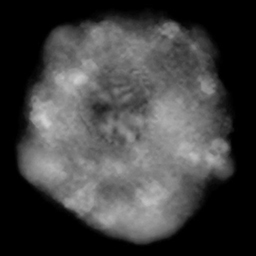
\includegraphics[width=0.22\columnwidth]{mypreprocess/orig/188gray}
		\label{fig:188none}
	}
	\subfigure[Image 1 after CEDORI. $\sigma=1.0$, $\rho=1.5$, $n=2$, $\tau=0.0015$.]
	{
		\includegraphics[width=0.22\columnwidth]{mypreprocess/cedori/188ced}
		\label{fig:188ced}
	}
	\subfigure[Image 1 after TV denoising. $\lambda=1.0$, $\epsilon=1\times10^{-3}$, $\gamma=20$.]
	{
		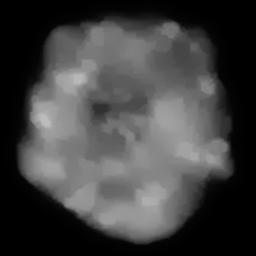
\includegraphics[width=0.22\columnwidth]{mypreprocess/tv/188graytv}
		\label{fig:188tv}
	}
	\subfigure[Image 1 after Proposed Pre-processing scheme. $\kappa_1=0.17$, $\kappa_2=0.55$, $R_1=50$, $R_2=225$,$N=50$.]
	{
		\includegraphics[width=0.22\columnwidth]{mypreprocess/proposed/188ced}
		\label{fig:188prop}
	}

	\subfigure[Original segmentation.]
	{
		\includegraphics[width=0.22\columnwidth]{mypreprocess/origseg/def188}
		\label{fig:188noneseg}
	}
	\subfigure[CEDORI segmentation.]
	{
		\includegraphics[width=0.22\columnwidth]{mypreprocess/cedseg/def188}
		\label{fig:188cedseg}
	}
	\subfigure[Total Variation Denoising segmentation.]
	{
		\includegraphics[width=0.22\columnwidth]{mypreprocess/tvseg/def188}
		\label{fig:188tvseg}
	}
	\subfigure[Proposed Pre-process segmentation.]
	{
		\includegraphics[width=0.22\columnwidth]{mypreprocess/proposedseg/def188}
		\label{fig:188propseg}
	}
	\caption{Image 1 from test set \Cref{AppendixA} pre-processing segmentation results. $\mu=1$, $\lambda_0=240$, $\lambda_1=8$.}
	\label{fig:preprocessschemeresult188}
\end{figure}

%%%%%%%%%%%%%%%%%%%%%%%%%%%%%%%%%%%%%%%%%%%%%%%%%%%%%%%
% 195
\begin{figure}[!h]
	\centering
	\subfigure[Image 2 without any pre-processing.]
	{
		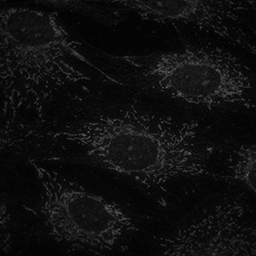
\includegraphics[width=0.22\columnwidth]{mypreprocess/orig/195gray}
		\label{fig:195none}
	}
	\subfigure[Image 2 after CEDORI. $\sigma=0.5$, $\rho=1.0$, $n=1$, $\tau=0.0005$.]
	{
		\includegraphics[width=0.22\columnwidth]{mypreprocess/cedori/195ced}
		\label{fig:195ced}
	}
	\subfigure[Image 2 after TV denoising. $\lambda=1.0$, $\epsilon=1\times10^{-3}$, $\gamma=5$.]
	{
		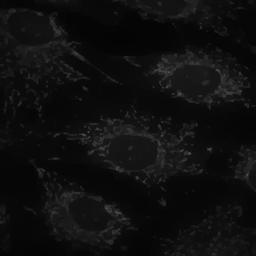
\includegraphics[width=0.22\columnwidth]{mypreprocess/tv/195graytv}
		\label{fig:195tv}
	}
	\subfigure[Image 2 after Proposed Pre-processing scheme. $\kappa_1=0.17$, $\kappa_2=0.55$, $R_1=50$, $R_2=225$,$N=50$.]
	{
		\includegraphics[width=0.22\columnwidth]{mypreprocess/proposed/195ced}
		\label{fig:195prop}
	}
	
	\subfigure[Original segmentation.]
	{
		\includegraphics[width=0.22\columnwidth]{mypreprocess/origseg/def195}
		\label{fig:195noneseg}
	}
	\subfigure[CEDORI segmentation.]
	{
		\includegraphics[width=0.22\columnwidth]{mypreprocess/cedseg/def195}
		\label{fig:195cedseg}
	}
	\subfigure[Total Variation Denoising segmentation.]
	{
		\includegraphics[width=0.22\columnwidth]{mypreprocess/tvseg/def195}
		\label{fig:195tvseg}
	}
	\subfigure[Proposed Pre-process segmentation.]
	{
		\includegraphics[width=0.22\columnwidth]{mypreprocess/proposedseg/def195}
		\label{fig:195propseg}
	}
	\caption{Image 2 from test set \Cref{AppendixA} pre-processing segmentation results. $\mu=1$, $\lambda_0=5$, $\lambda_1=1$.}
	\label{fig:preprocessschemeresult195}
\end{figure}

%%%%%%%%%%%%%%%%%%%%%%%%%%%%%%%%%%%%%%%%%%%%%%%%%%%%%%%
% 228
\begin{figure}[!h]
	\centering
	\subfigure[Image 3 without any pre-processing.]
	{
		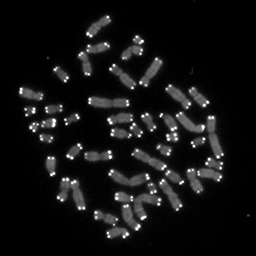
\includegraphics[width=0.22\columnwidth]{mypreprocess/orig/228gray}
		\label{fig:228none}
	}
	\subfigure[Image 3 after CEDORI. $\sigma=0.5$, $\rho=1.5$, $n=2$, $\tau=0.0005$.]
	{
		\includegraphics[width=0.22\columnwidth]{mypreprocess/cedori/228ced}
		\label{fig:228ced}
	}
	\subfigure[Image 3 after TV denoising. $\lambda=1.0$, $\epsilon=1\times10^{-3}$, $\gamma=20$.]
	{
		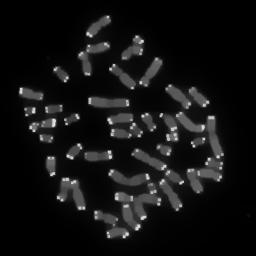
\includegraphics[width=0.22\columnwidth]{mypreprocess/tv/228graytv}
		\label{fig:228tv}
	}
	\subfigure[Image 3 after Proposed Pre-processing scheme. $\kappa_1=0.17$, $\kappa_2=0.55$, $R_1=50$, $R_2=225$,$N=50$.]
	{
		\includegraphics[width=0.22\columnwidth]{mypreprocess/proposed/228ced}
		\label{fig:228prop}
	}
	
	\subfigure[Original segmentation.]
	{
		\includegraphics[width=0.22\columnwidth]{mypreprocess/origseg/def228}
		\label{fig:228noneseg}
	}
	\subfigure[CEDORI segmentation.]
	{
		\includegraphics[width=0.22\columnwidth]{mypreprocess/cedseg/def228}
		\label{fig:228cedseg}
	}
	\subfigure[Total Variation Denoising segmentation.]
	{
		\includegraphics[width=0.22\columnwidth]{mypreprocess/tvseg/def228}
		\label{fig:228tvseg}
	}
	\subfigure[Proposed Pre-process segmentation.]
	{
		\includegraphics[width=0.22\columnwidth]{mypreprocess/proposedseg/def228}
		\label{fig:228propseg}
	}
	\caption{Image 3 from test set \Cref{AppendixA} pre-processing segmentation results. $\mu=1$, $\lambda_0=240$, $\lambda_1=8$.}
	\label{fig:preprocessschemeresult228}
\end{figure}

%%%%%%%%%%%%%%%%%%%%%%%%%%%%%%%%%%%%%%%%%%%%%%%%%%%%%%%
% 1057
\begin{figure}[!h]
	\centering
	\subfigure[Image 4 without any pre-processing.]
	{
		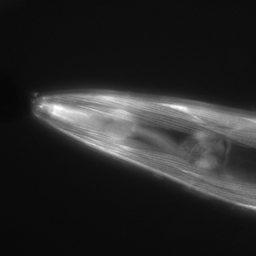
\includegraphics[width=0.22\columnwidth]{mypreprocess/orig/1057gray}
		\label{fig:1057none}
	}
	\subfigure[Image 4 after CEDORI. $\sigma=1.5$, $\rho=2.0$, $n=5$, $\tau=0.0015$.]
	{
		\includegraphics[width=0.22\columnwidth]{mypreprocess/cedori/1057ced}
		\label{fig:1057ced}
	}
	\subfigure[Image 4 after TV denoising. $\lambda=1.0$, $\epsilon=1\times10^{-3}$, $\gamma=20$.]
	{
		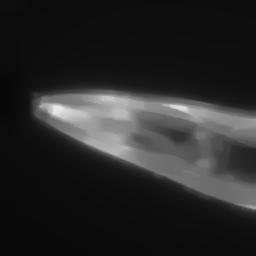
\includegraphics[width=0.22\columnwidth]{mypreprocess/tv/1057graytv}
		\label{fig:1057tv}
	}
	\subfigure[Image 4 after Proposed Pre-processing scheme. $\kappa_1=0.17$, $\kappa_2=0.55$, $R_1=50$, $R_2=225$,$N=50$.]
	{
		\includegraphics[width=0.22\columnwidth]{mypreprocess/proposed/1057ced}
		\label{fig:1057prop}
	}
	
	\subfigure[Original segmentation.]
	{
		\includegraphics[width=0.22\columnwidth]{mypreprocess/origseg/def1057}
		\label{fig:1057noneseg}
	}
	\subfigure[CEDORI segmentation.]
	{
		\includegraphics[width=0.22\columnwidth]{mypreprocess/cedseg/def1057}
		\label{fig:1057cedseg}
	}
	\subfigure[Total Variation Denoising segmentation.]
	{
		\includegraphics[width=0.22\columnwidth]{mypreprocess/tvseg/def1057}
		\label{fig:1057tvseg}
	}
	\subfigure[Proposed Pre-process segmentation.]
	{
		\includegraphics[width=0.22\columnwidth]{mypreprocess/proposedseg/def1057}
		\label{fig:1057propseg}
	}
	\caption{Image 4 from test set \Cref{AppendixA} pre-processing segmentation results. $\mu=1$, $\lambda_0=300$, $\lambda_1=5$.}
	\label{fig:preprocessschemeresult1057}
\end{figure}

%%%%%%%%%%%%%%%%%%%%%%%%%%%%%%%%%%%%%%%%%%%%%%%%%%%%%%%
% 1265
\begin{figure}[!h]
	\centering
	\subfigure[Image 5 without any pre-processing.]
	{
		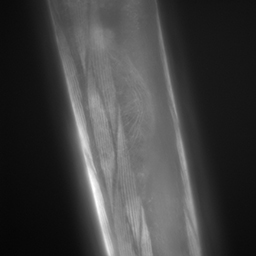
\includegraphics[width=0.22\columnwidth]{mypreprocess/orig/1265gray}
		\label{fig:1265none}
	}
	\subfigure[Image 5 after CEDORI. $\sigma=1.5$, $\rho=2.0$, $n=5$, $\tau=0.0015$.]
	{
		\includegraphics[width=0.22\columnwidth]{mypreprocess/cedori/1265ced}
		\label{fig:1265ced}
	}
	\subfigure[Image 5 after TV denoising. $\lambda=1.0$, $\epsilon=1\times10^{-3}$, $\gamma=20$.]
	{
		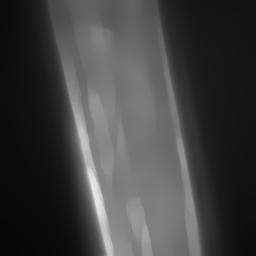
\includegraphics[width=0.22\columnwidth]{mypreprocess/tv/1265graytv}
		\label{fig1265tv}
	}
	\subfigure[Image 5 after Proposed Pre-processing scheme. $\kappa_1=0.17$, $\kappa_2=0.55$, $R_1=50$, $R_2=225$,$N=50$.]
	{
		\includegraphics[width=0.22\columnwidth]{mypreprocess/proposed/1265ced}
		\label{fig:1265prop}
	}
	
	\subfigure[Original segmentation.]
	{
		\includegraphics[width=0.22\columnwidth]{mypreprocess/origseg/def1265}
		\label{fig:1265noneseg}
	}
	\subfigure[CEDORI segmentation.]
	{
		\includegraphics[width=0.22\columnwidth]{mypreprocess/cedseg/def1265}
		\label{fig:1265cedseg}
	}
	\subfigure[Total Variation Denoising segmentation.]
	{
		\includegraphics[width=0.22\columnwidth]{mypreprocess/tvseg/def1265}
		\label{fig:1265tvseg}
	}
	\subfigure[Proposed Pre-process segmentation.]
	{
		\includegraphics[width=0.22\columnwidth]{mypreprocess/proposedseg/def1265}
		\label{fig:1265propseg}
	}
	\caption{Image 5 from test set \Cref{AppendixA} pre-processing segmentation results. $\mu=1$, $\lambda_0=220$, $\lambda_1=11$.}
	\label{fig:preprocessschemeresult1265}
\end{figure}

%%%%%%%%%%%%%%%%%%%%%%%%%%%%%%%%%%%%%%%%%%%%%%%%%%%%%%%
% 10093
\begin{figure}[!h]
	\centering
	\subfigure[Image 6 without any pre-processing.]
	{
		\includegraphics[width=0.22\columnwidth]{mypreprocess/orig/10093gray}
		\label{fig:10093none}
	}
	\subfigure[Image 6 after CEDORI. $\sigma=3.0$, $\rho=5.0$, $n=20$, $\tau=0.00075$.]
	{
		\includegraphics[width=0.22\columnwidth]{mypreprocess/cedori/10093ced}
		\label{fig:10093ced}
	}
	\subfigure[Image 6 after TV denoising. $\lambda=1.0$, $\epsilon=1\times10^{-3}$, $\gamma=20$.]
	{
		\includegraphics[width=0.22\columnwidth]{mypreprocess/tv/10093graytv}
		\label{fig:10093tv}
	}
	\subfigure[Image 6 after Proposed Pre-processing scheme. $\kappa_1=0.17$, $\kappa_2=0.65$, $R_1=12$, $R_2=225$,$N=12$.]
	{
		\includegraphics[width=0.22\columnwidth]{mypreprocess/proposed/10093ced}
		\label{fig:10093prop}
	}
	
	\subfigure[Original segmentation.]
	{
		\includegraphics[width=0.22\columnwidth]{mypreprocess/origseg/def10093}
		\label{fig:10093noneseg}
	}
	\subfigure[CEDORI segmentation.]
	{
		\includegraphics[width=0.22\columnwidth]{mypreprocess/cedseg/def10093}
		\label{fig:10093cedseg}
	}
	\subfigure[Total Variation Denoising segmentation.]
	{
		\includegraphics[width=0.22\columnwidth]{mypreprocess/tvseg/def10093}
		\label{fig:10093tvseg}
	}
	\subfigure[Proposed Pre-process segmentation.]
	{
		\includegraphics[width=0.22\columnwidth]{mypreprocess/proposedseg/def10093}
		\label{fig:10093propseg}
	}
	\caption{Image 6 from test set \Cref{AppendixA} pre-processing segmentation results. $\mu=1$, $\lambda_0=1600$, $\lambda_1=80$.}
	\label{fig:preprocessschemeresult10093}
\end{figure}

%%%%%%%%%%%%%%%%%%%%%%%%%%%%%%%%%%%%%%%%%%%%%%%%%%%%%%%
% 10093
\begin{figure}[!h]
	\centering
	\subfigure[Image 7 without any pre-processing.]
	{
		\includegraphics[width=0.22\columnwidth]{mypreprocess/orig/10102gray}
		\label{fig:10102none}
	}
	\subfigure[Image 7 after CEDORI. $\sigma=3.0$, $\rho=3.0$, $n=20$, $\tau=0.00075$.]
	{
		\includegraphics[width=0.22\columnwidth]{mypreprocess/cedori/10102ced}
		\label{fig:10102ced}
	}
	\subfigure[Image 7 after TV denoising. $\lambda=1.0$, $\epsilon=1\times10^{-3}$, $\gamma=20$.]
	{
		\includegraphics[width=0.22\columnwidth]{mypreprocess/tv/10102graytv}
		\label{fig:10102tv}
	}
	\subfigure[Image 7 after Proposed Pre-processing scheme. $\kappa_1=0.17$, $\kappa_2=0.65$, $R_1=12$, $R_2=225$,$N=12$.]
	{
		\includegraphics[width=0.22\columnwidth]{mypreprocess/proposed/10102ced}
		\label{fig:10102prop}
	}
	
	\subfigure[Original segmentation.]
	{
		\includegraphics[width=0.22\columnwidth]{mypreprocess/origseg/def10102}
		\label{fig:10102noneseg}
	}
	\subfigure[CEDORI segmentation.]
	{
		\includegraphics[width=0.22\columnwidth]{mypreprocess/cedseg/def10102}
		\label{fig:10102cedseg}
	}
	\subfigure[Total Variation Denoising segmentation.]
	{
		\includegraphics[width=0.22\columnwidth]{mypreprocess/tvseg/def10102}
		\label{fig:10102tvseg}
	}
	\subfigure[Proposed Pre-process segmentation.]
	{
		\includegraphics[width=0.22\columnwidth]{mypreprocess/proposedseg/def10102}
		\label{fig:10102propseg}
	}
	\caption{Image 7 from test set \Cref{AppendixA} pre-processing segmentation results. $\mu=1$, $\lambda_0=10$, $\lambda_1=1$.}
	\label{fig:preprocessschemeresult101023}
\end{figure}

%%%%%%%%%%%%%%%%%%%%%%%%%%%%%%%%%%%%%%%%%%%%%%%%%%%%%%%
% 10104
\begin{figure}[!h]
	\centering
	\subfigure[Image 8 without any pre-processing.]
	{
		\includegraphics[width=0.22\columnwidth]{mypreprocess/orig/10104gray}
		\label{fig:10104none}
	}
	\subfigure[Image 8 after CEDORI. $\sigma=3.0$, $\rho=3.0$, $n=20$, $\tau=0.00075$.]
	{
		\includegraphics[width=0.22\columnwidth]{mypreprocess/cedori/10104ced}
		\label{fig:10104ced}
	}
	\subfigure[Image 8 after TV denoising. $\lambda=1.0$, $\epsilon=1\times10^{-3}$, $\gamma=20$.]
	{
		\includegraphics[width=0.22\columnwidth]{mypreprocess/tv/10104graytv}
		\label{fig:10104tv}
	}
	\subfigure[Image 8 after Proposed Pre-processing scheme. $\kappa_1=0.17$, $\kappa_2=0.65$, $R_1=12$, $R_2=225$,$N=12$.]
	{
		\includegraphics[width=0.22\columnwidth]{mypreprocess/proposed/10104ced}
		\label{fig:10104prop}
	}
	
	\subfigure[Original segmentation.]
	{
		\includegraphics[width=0.22\columnwidth]{mypreprocess/origseg/def10104}
		\label{fig:10104noneseg}
	}
	\subfigure[CEDORI segmentation.]
	{
		\includegraphics[width=0.22\columnwidth]{mypreprocess/cedseg/def10104}
		\label{fig:10104cedseg}
	}
	\subfigure[Total Variation Denoising segmentation.]
	{
		\includegraphics[width=0.22\columnwidth]{mypreprocess/tvseg/def10104}
		\label{fig:10104tvseg}
	}
	\subfigure[Proposed Pre-process segmentation.]
	{
		\includegraphics[width=0.22\columnwidth]{mypreprocess/proposedseg/def10104}
		\label{fig:10104propseg}
	}
	\caption{Image 8 from test set \Cref{AppendixA} pre-processing segmentation results. $\mu=1$, $\lambda_0=10$, $\lambda_1=1$.}
	\label{fig:preprocessschemeresult10104}
\end{figure}

%%%%%%%%%%%%%%%%%%%%%%%%%%%%%%%%%%%%%%%%%%%%%%%%%%%%%%%
% 12294
\begin{figure}[!h]
	\centering
	\subfigure[Image 9 without any pre-processing.]
	{
		\includegraphics[width=0.22\columnwidth]{mypreprocess/orig/12294gray}
		\label{fig:12294none}
	}
	\subfigure[Image 9 after CEDORI. $\sigma=0.5$, $\rho=1.0$, $n=2$, $\tau=0.0005$.]
	{
		\includegraphics[width=0.22\columnwidth]{mypreprocess/cedori/12294ced}
		\label{fig:12294ced}
	}
	\subfigure[Image 9 after TV denoising. $\lambda=1.0$, $\epsilon=1\times10^{-3}$, $\gamma=5$.]
	{
		\includegraphics[width=0.22\columnwidth]{mypreprocess/tv/12294graytv}
		\label{fig:12294tv}
	}
	\subfigure[Image 9 after Proposed Pre-processing scheme. $\kappa_1=0.17$, $\kappa_2=0.65$, $R_1=12$, $R_2=225$,$N=12$.]
	{
		\includegraphics[width=0.22\columnwidth]{mypreprocess/proposed/12294ced}
		\label{fig:12294prop}
	}
	
	\subfigure[Original segmentation.]
	{
		\includegraphics[width=0.22\columnwidth]{mypreprocess/origseg/def12294}
		\label{fig:12294noneseg}
	}
	\subfigure[CEDORI segmentation.]
	{
		\includegraphics[width=0.22\columnwidth]{mypreprocess/cedseg/def12294}
		\label{fig:12294cedseg}
	}
	\subfigure[Total Variation Denoising segmentation.]
	{
		\includegraphics[width=0.22\columnwidth]{mypreprocess/tvseg/def12294}
		\label{fig:12294tvseg}
	}
	\subfigure[Proposed Pre-process segmentation.]
	{
		\includegraphics[width=0.22\columnwidth]{mypreprocess/proposedseg/def12294}
		\label{fig:12294propseg}
	}
	\caption{Image 9 from test set \Cref{AppendixA} pre-processing segmentation results. $\mu=1$, $\lambda_0=2700$, $\lambda_1=90$.}
	\label{fig:preprocessschemeresult12294}
\end{figure}

%%%%%%%%%%%%%%%%%%%%%%%%%%%%%%%%%%%%%%%%%%%%%%%%%%%%%%%
% 12627
\begin{figure}[!h]
	\centering
	\subfigure[Image 10 without any pre-processing.]
	{
		\includegraphics[width=0.22\columnwidth]{mypreprocess/orig/12627gray}
		\label{fig:12627none}
	}
	\subfigure[Image 10 after CEDORI. $\sigma=3.0$, $\rho=5.0$, $n=10$, $\tau=0.0005$.]
	{
		\includegraphics[width=0.22\columnwidth]{mypreprocess/cedori/12627ced}
		\label{fig:12627ced}
	}
	\subfigure[Image 10 after TV denoising. $\lambda=1.0$, $\epsilon=1\times10^{-3}$, $\gamma=20$.]
	{
		\includegraphics[width=0.22\columnwidth]{mypreprocess/tv/12627graytv}
		\label{fig:12627tv}
	}
	\subfigure[Image 10 after Proposed Pre-processing scheme. $\kappa_1=0.17$, $\kappa_2=0.65$, $R_1=12$, $R_2=225$,$N=12$.]
	{
		\includegraphics[width=0.22\columnwidth]{mypreprocess/proposed/12627ced}
		\label{fig:12627prop}
	}
	
	\subfigure[Original segmentation.]
	{
		\includegraphics[width=0.22\columnwidth]{mypreprocess/origseg/def12627}
		\label{fig:12627noneseg}
	}
	\subfigure[CEDORI segmentation.]
	{
		\includegraphics[width=0.22\columnwidth]{mypreprocess/cedseg/def12627}
		\label{fig:12627cedseg}
	}
	\subfigure[Total Variation Denoising segmentation.]
	{
		\includegraphics[width=0.22\columnwidth]{mypreprocess/tvseg/def12627}
		\label{fig:12627tvseg}
	}
	\subfigure[Proposed Pre-process segmentation.]
	{
		\includegraphics[width=0.22\columnwidth]{mypreprocess/proposedseg/def12627}
		\label{fig:12627propseg}
	}
	\caption{Image 10 from test set \Cref{AppendixA} pre-processing segmentation results. $\mu=1$, $\lambda_0=4050$, $\lambda_1=135$.}
	\label{fig:preprocessschemeresult12627}
\end{figure}

%%%%%%%%%%%%%%%%%%%%%%%%%%%%%%%%%%%%%%%%%%%%%%%%%%%%%%%
% 13432
\begin{figure}[!h]
	\centering
	\subfigure[Image 11 without any pre-processing.]
	{
		\includegraphics[width=0.22\columnwidth]{mypreprocess/orig/13432gray}
		\label{fig:13432none}
	}
	\subfigure[Image 11 after CEDORI. $\sigma=1.0$, $\rho=1.0$, $n=1$, $\tau=0.0005$.]
	{
		\includegraphics[width=0.22\columnwidth]{mypreprocess/cedori/13432ced}
		\label{fig:13432ced}
	}
	\subfigure[Image 11 after TV denoising. $\lambda=1.0$, $\epsilon=1\times10^{-3}$, $\gamma=20$.]
	{
		\includegraphics[width=0.22\columnwidth]{mypreprocess/tv/13432graytv}
		\label{fig:13432tv}
	}
	\subfigure[Image 11 after Proposed Pre-processing scheme. $\kappa_1=0.17$, $\kappa_2=0.55$, $R_1=50$, $R_2=225$,$N=50$.]
	{
		\includegraphics[width=0.22\columnwidth]{mypreprocess/proposed/13432ced}
		\label{fig:13432prop}
	}
	
	\subfigure[Original segmentation.]
	{
		\includegraphics[width=0.22\columnwidth]{mypreprocess/origseg/def13432}
		\label{fig:13432noneseg}
	}
	\subfigure[CEDORI segmentation.]
	{
		\includegraphics[width=0.22\columnwidth]{mypreprocess/cedseg/def13432}
		\label{fig:13432cedseg}
	}
	\subfigure[Total Variation Denoising segmentation.]
	{
		\includegraphics[width=0.22\columnwidth]{mypreprocess/tvseg/def13432}
		\label{fig:13432tvseg}
	}
	\subfigure[Proposed Pre-process segmentation.]
	{
		\includegraphics[width=0.22\columnwidth]{mypreprocess/proposedseg/def13432}
		\label{fig:13432propseg}
	}
	\caption{Image 11 from test set \Cref{AppendixA} pre-processing segmentation results. $\mu=1$, $\lambda_0=10$, $\lambda_1=1$.}
	\label{fig:preprocessschemeresult13432}
\end{figure}

%%%%%%%%%%%%%%%%%%%%%%%%%%%%%%%%%%%%%%%%%%%%%%%%%%%%%%%
% 13438
\begin{figure}[!h]
	\centering
	\subfigure[Image 12 without any pre-processing.]
	{
		\includegraphics[width=0.22\columnwidth]{mypreprocess/orig/13438gray}
		\label{fig:13438none}
	}
	\subfigure[Image 12 after CEDORI. $\sigma=0.5$, $\rho=1.0$, $n=10$, $\tau=0.0005$.]
	{
		\includegraphics[width=0.22\columnwidth]{mypreprocess/cedori/13438ced}
		\label{fig:13438ced}
	}
	\subfigure[Image 12 after TV denoising. $\lambda=1.0$, $\epsilon=1\times10^{-3}$, $\gamma=20$.]
	{
		\includegraphics[width=0.22\columnwidth]{mypreprocess/tv/13438graytv}
		\label{fig:13438tv}
	}
	\subfigure[Image 12 after Proposed Pre-processing scheme. $\kappa_1=0.17$, $\kappa_2=0.55$, $R_1=50$, $R_2=225$,$N=50$.]
	{
		\includegraphics[width=0.22\columnwidth]{mypreprocess/proposed/13438ced}
		\label{fig:13438prop}
	}
	
	\subfigure[Original segmentation.]
	{
		\includegraphics[width=0.22\columnwidth]{mypreprocess/origseg/def13438}
		\label{fig:13438noneseg}
	}
	\subfigure[CEDORI segmentation.]
	{
		\includegraphics[width=0.22\columnwidth]{mypreprocess/cedseg/def13438}
		\label{fig:13438cedseg}
	}
	\subfigure[Total Variation Denoising segmentation.]
	{
		\includegraphics[width=0.22\columnwidth]{mypreprocess/tvseg/def13438}
		\label{fig:13438tvseg}
	}
	\subfigure[Proposed Pre-process segmentation.]
	{
		\includegraphics[width=0.22\columnwidth]{mypreprocess/proposedseg/def13438}
		\label{fig:13438propseg}
	}
	\caption{Image 12 from test set \Cref{AppendixA} pre-processing segmentation results. $\mu=1$, $\lambda_0=10$, $\lambda_1=1$.}
	\label{fig:preprocessschemeresult13438}
\end{figure}

%%%%%%%%%%%%%%%%%%%%%%%%%%%%%%%%%%%%%%%%%%%%%%%%%%%%%%%
% 13899
\begin{figure}[!h]
	\centering
	\subfigure[Image 13 without any pre-processing.]
	{
		\includegraphics[width=0.22\columnwidth]{mypreprocess/orig/13899gray}
		\label{fig:13899none}
	}
	\subfigure[Image 13 after CEDORI. $\sigma=0.5$, $\rho=1.0$, $n=20$, $\tau=0.0001$.]
	{
		\includegraphics[width=0.22\columnwidth]{mypreprocess/cedori/13899ced}
		\label{fig:13899ced}
	}
	\subfigure[Image 13 after TV denoising. $\lambda=1.0$, $\epsilon=1\times10^{-3}$, $\gamma=20$.]
	{
		\includegraphics[width=0.22\columnwidth]{mypreprocess/tv/13899graytv}
		\label{fig:13899tv}
	}
	\subfigure[Image 13 after Proposed Pre-processing scheme. $\kappa_1=0.17$, $\kappa_2=0.55$, $R_1=50$, $R_2=225$,$N=50$.]
	{
		\includegraphics[width=0.22\columnwidth]{mypreprocess/proposed/13899ced}
		\label{fig:13899prop}
	}
	
	\subfigure[Original segmentation.]
	{
		\includegraphics[width=0.22\columnwidth]{mypreprocess/origseg/def13899}
		\label{fig:13899noneseg}
	}
	\subfigure[CEDORI segmentation.]
	{
		\includegraphics[width=0.22\columnwidth]{mypreprocess/cedseg/def13899}
		\label{fig:13899cedseg}
	}
	\subfigure[Total Variation Denoising segmentation.]
	{
		\includegraphics[width=0.22\columnwidth]{mypreprocess/tvseg/def13899}
		\label{fig:13899tvseg}
	}
	\subfigure[Proposed Pre-process segmentation.]
	{
		\includegraphics[width=0.22\columnwidth]{mypreprocess/proposedseg/def13899}
		\label{fig:13899propseg}
	}
	\caption{Image 13 from test set \Cref{AppendixA} pre-processing segmentation results. $\mu=1$, $\lambda_0=10$, $\lambda_1=1$.}
	\label{fig:preprocessschemeresult13899}
\end{figure}

%%%%%%%%%%%%%%%%%%%%%%%%%%%%%%%%%%%%%%%%%%%%%%%%%%%%%%%
% 13901
\begin{figure}[!h]
	\centering
	\subfigure[Image 14 without any pre-processing.]
	{
		\includegraphics[width=0.22\columnwidth]{mypreprocess/orig/13901gray}
		\label{fig:13901none}
	}
	\subfigure[Image 14 after CEDORI. $\sigma=1.0$, $\rho=1.0$, $n=5$, $\tau=0.0001$.]
	{
		\includegraphics[width=0.22\columnwidth]{mypreprocess/cedori/13901ced}
		\label{fig:13901ced}
	}
	\subfigure[Image 14 after TV denoising. $\lambda=1.0$, $\epsilon=1\times10^{-3}$, $\gamma=20$.]
	{
		\includegraphics[width=0.22\columnwidth]{mypreprocess/tv/13901graytv}
		\label{fig:13901tv}
	}
	\subfigure[Image 14 after Proposed Pre-processing scheme. $\kappa_1=0.17$, $\kappa_2=0.55$, $R_1=50$, $R_2=225$,$N=50$.]
	{
		\includegraphics[width=0.22\columnwidth]{mypreprocess/proposed/13901ced}
		\label{fig:13901prop}
	}
	
	\subfigure[Original segmentation.]
	{
		\includegraphics[width=0.22\columnwidth]{mypreprocess/origseg/def13901}
		\label{fig:13901noneseg}
	}
	\subfigure[CEDORI segmentation.]
	{
		\includegraphics[width=0.22\columnwidth]{mypreprocess/cedseg/def13901}
		\label{fig:13901cedseg}
	}
	\subfigure[Total Variation Denoising segmentation.]
	{
		\includegraphics[width=0.22\columnwidth]{mypreprocess/tvseg/def13901}
		\label{fig:13901tvseg}
	}
	\subfigure[Proposed Pre-process segmentation.]
	{
		\includegraphics[width=0.22\columnwidth]{mypreprocess/proposedseg/def13901}
		\label{fig:13901propseg}
	}
	\caption{Image 14 from test set \Cref{AppendixA} pre-processing segmentation results. $\mu=1$, $\lambda_0=3$, $\lambda_1=1$.}
	\label{fig:preprocessschemeresult13901}
\end{figure}

%%%%%%%%%%%%%%%%%%%%%%%%%%%%%%%%%%%%%%%%%%%%%%%%%%%%%%%
% 21749
\begin{figure}[!h]
	\centering
	\subfigure[Image 15 without any pre-processing.]
	{
		\includegraphics[width=0.22\columnwidth]{mypreprocess/orig/21749gray}
		\label{fig:21749none}
	}
	\subfigure[Image 15 after CEDORI. $\sigma=1.0$, $\rho=1.0$, $n=20$, $\tau=0.0005$.]
	{
		\includegraphics[width=0.22\columnwidth]{mypreprocess/cedori/21749ced}
		\label{fig:21749ced}
	}
	\subfigure[Image 15 after TV denoising. $\lambda=1.0$, $\epsilon=1\times10^{-3}$, $\gamma=20$.]
	{
		\includegraphics[width=0.22\columnwidth]{mypreprocess/tv/21749graytv}
		\label{fig:21749tv}
	}
	\subfigure[Image 15 after Proposed Pre-processing scheme. $\kappa_1=0.17$, $\kappa_2=0.65$, $R_1=12$, $R_2=225$,$N=12$.]
	{
		\includegraphics[width=0.22\columnwidth]{mypreprocess/proposed/21749ced}
		\label{fig:21749prop}
	}
	
	\subfigure[Original segmentation.]
	{
		\includegraphics[width=0.22\columnwidth]{mypreprocess/origseg/def21749}
		\label{fig:21749noneseg}
	}
	\subfigure[CEDORI segmentation.]
	{
		\includegraphics[width=0.22\columnwidth]{mypreprocess/cedseg/def21749}
		\label{fig:21749cedseg}
	}
	\subfigure[Total Variation Denoising segmentation.]
	{
		\includegraphics[width=0.22\columnwidth]{mypreprocess/tvseg/def21749}
		\label{fig:21749tvseg}
	}
	\subfigure[Proposed Pre-process segmentation.]
	{
		\includegraphics[width=0.22\columnwidth]{mypreprocess/proposedseg/def21749}
		\label{fig:21749propseg}
	}
	\caption{Image 15 from test set \Cref{AppendixA} pre-processing segmentation results. $\mu=1$, $\lambda_0=10$, $\lambda_1=1$.}
	\label{fig:preprocessschemeresult21749}
\end{figure}

%%%%%%%%%%%%%%%%%%%%%%%%%%%%%%%%%%%%%%%%%%%%%%%%%%%%%%%
% 21759
\begin{figure}[!h]
	\centering
	\subfigure[Image 16 without any pre-processing.]
	{
		\includegraphics[width=0.22\columnwidth]{mypreprocess/orig/21759gray}
		\label{fig:21759none}
	}
	\subfigure[Image 16 after CEDORI. $\sigma=3.0$, $\rho=1.0$, $n=20$, $\tau=0.0005$.]
	{
		\includegraphics[width=0.22\columnwidth]{mypreprocess/cedori/21759ced}
		\label{fig:21759ced}
	}
	\subfigure[Image 16 after TV denoising. $\lambda=1.0$, $\epsilon=1\times10^{-3}$, $\gamma=20$.]
	{
		\includegraphics[width=0.22\columnwidth]{mypreprocess/tv/21759graytv}
		\label{fig:21759tv}
	}
	\subfigure[Image 16 after Proposed Pre-processing scheme. $\kappa_1=0.17$, $\kappa_2=0.55$, $R_1=50$, $R_2=225$,$N=50$.]
	{
		\includegraphics[width=0.22\columnwidth]{mypreprocess/proposed/21759ced}
		\label{fig:21759prop}
	}
	
	\subfigure[Original segmentation.]
	{
		\includegraphics[width=0.22\columnwidth]{mypreprocess/origseg/def21759}
		\label{fig:21759noneseg}
	}
	\subfigure[CEDORI segmentation.]
	{
		\includegraphics[width=0.22\columnwidth]{mypreprocess/cedseg/def21759}
		\label{fig:21759cedseg}
	}
	\subfigure[Total Variation Denoising segmentation.]
	{
		\includegraphics[width=0.22\columnwidth]{mypreprocess/tvseg/def21759}
		\label{fig:21759tvseg}
	}
	\subfigure[Proposed Pre-process segmentation.]
	{
		\includegraphics[width=0.22\columnwidth]{mypreprocess/proposedseg/def21759}
		\label{fig:21759propseg}
	}
	\caption{Image 16 from test set \Cref{AppendixA} pre-processing segmentation results. $\mu=1$, $\lambda_0=10$, $\lambda_1=1$.}
	\label{fig:preprocessschemeresult21759}
\end{figure}

%%%%%%%%%%%%%%%%%%%%%%%%%%%%%%%%%%%%%%%%%%%%%%%%%%%%%%%
% 32140
\begin{figure}[!h]
	\centering
	\subfigure[Image 17 without any pre-processing.]
	{
		\includegraphics[width=0.22\columnwidth]{mypreprocess/orig/32140gray}
		\label{fig:32140none}
	}
	\subfigure[Image 17 after CEDORI. $\sigma=3.0$, $\rho=3.0$, $n=20$, $\tau=0.0005$.]
	{
		\includegraphics[width=0.22\columnwidth]{mypreprocess/cedori/32140ced}
		\label{fig:32140ced}
	}
	\subfigure[Image 17 after TV denoising. $\lambda=1.0$, $\epsilon=1\times10^{-3}$, $\gamma=20$.]
	{
		\includegraphics[width=0.22\columnwidth]{mypreprocess/tv/32140graytv}
		\label{fig:32140tv}
	}
	\subfigure[Image 17 after Proposed Pre-processing scheme. $\kappa_1=0.17$, $\kappa_2=0.55$, $R_1=50$, $R_2=225$,$N=50$.]
	{
		\includegraphics[width=0.22\columnwidth]{mypreprocess/proposed/32140ced}
		\label{fig:32140prop}
	}
	
	\subfigure[Original segmentation.]
	{
		\includegraphics[width=0.22\columnwidth]{mypreprocess/origseg/def32140}
		\label{fig:32140noneseg}
	}
	\subfigure[CEDORI segmentation.]
	{
		\includegraphics[width=0.22\columnwidth]{mypreprocess/cedseg/def32140}
		\label{fig:32140cedseg}
	}
	\subfigure[Total Variation Denoising segmentation.]
	{
		\includegraphics[width=0.22\columnwidth]{mypreprocess/tvseg/def32140}
		\label{fig:32140tvseg}
	}
	\subfigure[Proposed Pre-process segmentation.]
	{
		\includegraphics[width=0.22\columnwidth]{mypreprocess/proposedseg/def32140}
		\label{fig:32140propseg}
	}
	\caption{Image 17 from test set \Cref{AppendixA} pre-processing segmentation results. $\mu=1$, $\lambda_0=5$, $\lambda_1=1$.}
	\label{fig:preprocessschemeresult32140}
\end{figure}

%%%%%%%%%%%%%%%%%%%%%%%%%%%%%%%%%%%%%%%%%%%%%%%%%%%%%%%
% 35278
\begin{figure}[!h]
	\centering
	\subfigure[Image 18 without any pre-processing.]
	{
		\includegraphics[width=0.22\columnwidth]{mypreprocess/orig/35278gray}
		\label{fig:35278none}
	}
	\subfigure[Image 18 after CEDORI. $\sigma=1.0$, $\rho=1.0$, $n=20$, $\tau=0.0005$.]
	{
		\includegraphics[width=0.22\columnwidth]{mypreprocess/cedori/35278ced}
		\label{fig:35278ced}
	}
	\subfigure[Image 18 after TV denoising. $\lambda=1.0$, $\epsilon=1\times10^{-3}$, $\gamma=5$.]
	{
		\includegraphics[width=0.22\columnwidth]{mypreprocess/tv/35278graytv}
		\label{fig:35278tv}
	}
	\subfigure[Image 18 after Proposed Pre-processing scheme. $\kappa_1=0.17$, $\kappa_2=0.65$, $R_1=12$, $R_2=225$,$N=12$.]
	{
		\includegraphics[width=0.22\columnwidth]{mypreprocess/proposed/35278ced}
		\label{fig:35278prop}
	}
	
	\subfigure[Original segmentation.]
	{
		\includegraphics[width=0.22\columnwidth]{mypreprocess/origseg/def35278}
		\label{fig:35278noneseg}
	}
	\subfigure[CEDORI segmentation.]
	{
		\includegraphics[width=0.22\columnwidth]{mypreprocess/cedseg/def35278}
		\label{fig:35278cedseg}
	}
	\subfigure[Total Variation Denoising segmentation.]
	{
		\includegraphics[width=0.22\columnwidth]{mypreprocess/tvseg/def35278}
		\label{fig:35278tvseg}
	}
	\subfigure[Proposed Pre-process segmentation.]
	{
		\includegraphics[width=0.22\columnwidth]{mypreprocess/proposedseg/def35278}
		\label{fig:35278propseg}
	}
	\caption{Image 18 from test set \Cref{AppendixA} pre-processing segmentation results. $\mu=1$, $\lambda_0=5$, $\lambda_1=1$.}
	\label{fig:preprocessschemeresult35278}
\end{figure}

%%%%%%%%%%%%%%%%%%%%%%%%%%%%%%%%%%%%%%%%%%%%%%%%%%%%%%%
% 37338
\begin{figure}[!h]
	\centering
	\subfigure[Image 19 without any pre-processing.]
	{
		\includegraphics[width=0.22\columnwidth]{mypreprocess/orig/37338gray}
		\label{fig:37338none}
	}
	\subfigure[Image 19 after CEDORI. $\sigma=0.5$, $\rho=5.0$, $n=50$, $\tau=0.0002$.]
	{
		\includegraphics[width=0.22\columnwidth]{mypreprocess/cedori/37338ced}
		\label{fig:37338ced}
	}
	\subfigure[Image 19 after TV denoising. $\lambda=1.0$, $\epsilon=1\times10^{-3}$, $\gamma=20$.]
	{
		\includegraphics[width=0.22\columnwidth]{mypreprocess/tv/37338graytv}
		\label{fig:37338tv}
	}
	\subfigure[Image 19 after Proposed Pre-processing scheme. $\kappa_1=0.17$, $\kappa_2=0.65$, $R_1=12$, $R_2=225$,$N=12$.]
	{
		\includegraphics[width=0.22\columnwidth]{mypreprocess/proposed/37338ced}
		\label{fig:37338prop}
	}
	
	\subfigure[Original segmentation.]
	{
		\includegraphics[width=0.22\columnwidth]{mypreprocess/origseg/def37338}
		\label{fig:373388noneseg}
	}
	\subfigure[CEDORI segmentation.]
	{
		\includegraphics[width=0.22\columnwidth]{mypreprocess/cedseg/def37338}
		\label{fig:37338cedseg}
	}
	\subfigure[Total Variation Denoising segmentation.]
	{
		\includegraphics[width=0.22\columnwidth]{mypreprocess/tvseg/def37338}
		\label{fig:37338tvseg}
	}
	\subfigure[Proposed Pre-process segmentation.]
	{
		\includegraphics[width=0.22\columnwidth]{mypreprocess/proposedseg/def37338}
		\label{fig:37338propseg}
	}
	\caption{Image 19 from test set \Cref{AppendixA} pre-processing segmentation results. $\mu=1$, $\lambda_0=6$, $\lambda_1=2$.}
	\label{fig:preprocessschemeresult37338}
\end{figure}

%%%%%%%%%%%%%%%%%%%%%%%%%%%%%%%%%%%%%%%%%%%%%%%%%%%%%%%
% 37339
\begin{figure}[!h]
	\centering
	\subfigure[Image 20 without any pre-processing.]
	{
		\includegraphics[width=0.22\columnwidth]{mypreprocess/orig/37339gray}
		\label{fig:37339none}
	}
	\subfigure[Image 20 after CEDORI. $\sigma=0.5$, $\rho=5.0$, $n=50$, $\tau=0.0002$.]
	{
		\includegraphics[width=0.22\columnwidth]{mypreprocess/cedori/37339ced}
		\label{fig:37339ced}
	}
	\subfigure[Image 20 after TV denoising. $\lambda=1.0$, $\epsilon=1\times10^{-3}$, $\gamma=20$.]
	{
		\includegraphics[width=0.22\columnwidth]{mypreprocess/tv/37339graytv}
		\label{fig:37339tv}
	}
	\subfigure[Image 20 after Proposed Pre-processing scheme. $\kappa_1=0.17$, $\kappa_2=0.65$, $R_1=12$, $R_2=225$,$N=12$.]
	{
		\includegraphics[width=0.22\columnwidth]{mypreprocess/proposed/37339ced}
		\label{fig:37339prop}
	}
	
	\subfigure[Original segmentation.]
	{
		\includegraphics[width=0.22\columnwidth]{mypreprocess/origseg/def37339}
		\label{fig:37339noneseg}
	}
	\subfigure[CEDORI segmentation.]
	{
		\includegraphics[width=0.22\columnwidth]{mypreprocess/cedseg/def37339}
		\label{fig:37339cedseg}
	}
	\subfigure[Total Variation Denoising segmentation.]
	{
		\includegraphics[width=0.22\columnwidth]{mypreprocess/tvseg/def37339}
		\label{fig:37339tvseg}
	}
	\subfigure[Proposed Pre-process segmentation.]
	{
		\includegraphics[width=0.22\columnwidth]{mypreprocess/proposedseg/def37339}
		\label{fig:37339propseg}
	}
	\caption{Image 20 from test set \Cref{AppendixA} pre-processing segmentation results. $\mu=1$, $\lambda_0=6$, $\lambda_1=2$.}
	\label{fig:preprocessschemeresult37339}
\end{figure}

%%%%%%%%%%%%%%%%%%%%%%%%%%%%%%%%%%%%%%%%%%%%%%%%%%%%%%%
% 38974
\begin{figure}[!h]
	\centering
	\subfigure[Image 21 without any pre-processing.]
	{
		\includegraphics[width=0.22\columnwidth]{mypreprocess/orig/38974gray}
		\label{fig:38974none}
	}
	\subfigure[Image 21 after CEDORI. $\sigma=0.5$, $\rho=1.0$, $n=15$, $\tau=0.0005$.]
	{
		\includegraphics[width=0.22\columnwidth]{mypreprocess/cedori/38974ced}
		\label{fig:38974ced}
	}
	\subfigure[Image 21 after TV denoising. $\lambda=1.0$, $\epsilon=1\times10^{-3}$, $\gamma=5$.]
	{
		\includegraphics[width=0.22\columnwidth]{mypreprocess/tv/38974graytv}
		\label{fig:38974tv}
	}
	\subfigure[Image 21 after Proposed Pre-processing scheme. $\kappa_1=0.17$, $\kappa_2=0.55$, $R_1=50$, $R_2=225$,$N=50$.]
	{
		\includegraphics[width=0.22\columnwidth]{mypreprocess/proposed/38974ced}
		\label{fig:38974prop}
	}
	
	\subfigure[Original segmentation.]
	{
		\includegraphics[width=0.22\columnwidth]{mypreprocess/origseg/def38974}
		\label{fig:38974noneseg}
	}
	\subfigure[CEDORI segmentation.]
	{
		\includegraphics[width=0.22\columnwidth]{mypreprocess/cedseg/def38974}
		\label{fig:38974cedseg}
	}
	\subfigure[Total Variation Denoising segmentation.]
	{
		\includegraphics[width=0.22\columnwidth]{mypreprocess/tvseg/def38974}
		\label{fig:38974tvseg}
	}
	\subfigure[Proposed Pre-process segmentation.]
	{
		\includegraphics[width=0.22\columnwidth]{mypreprocess/proposedseg/def38974}
		\label{fig:38974propseg}
	}
	\caption{Image 21 from test set \Cref{AppendixA} pre-processing segmentation results. $\mu=1$, $\lambda_0=300$, $\lambda_1=30$.}
	\label{fig:preprocessschemeresult38974}
\end{figure}

%%%%%%%%%%%%%%%%%%%%%%%%%%%%%%%%%%%%%%%%%%%%%%%%%%%%%%%
% 40217
\begin{figure}[!h]
	\centering
	\subfigure[Image 22 without any pre-processing.]
	{
		\includegraphics[width=0.22\columnwidth]{mypreprocess/orig/40217gray}
		\label{fig:40217none}
	}
	\subfigure[Image 22 after CEDORI. $\sigma=1.0$, $\rho=1.0$, $n=20$, $\tau=0.0005$.]
	{
		\includegraphics[width=0.22\columnwidth]{mypreprocess/cedori/40217ced}
		\label{fig:40217ced}
	}
	\subfigure[Image 22 after TV denoising. $\lambda=1.0$, $\epsilon=1\times10^{-3}$, $\gamma=20$.]
	{
		\includegraphics[width=0.22\columnwidth]{mypreprocess/tv/40217graytv}
		\label{fig:40217tv}
	}
	\subfigure[Image 22 after Proposed Pre-processing scheme. $\kappa_1=0.17$, $\kappa_2=0.55$, $R_1=50$, $R_2=225$,$N=50$.]
	{
		\includegraphics[width=0.22\columnwidth]{mypreprocess/proposed/40217ced}
		\label{fig:40217prop}
	}
	
	\subfigure[Original segmentation.]
	{
		\includegraphics[width=0.22\columnwidth]{mypreprocess/origseg/def40217}
		\label{fig:40217noneseg}
	}
	\subfigure[CEDORI segmentation.]
	{
		\includegraphics[width=0.22\columnwidth]{mypreprocess/cedseg/def40217}
		\label{fig:40217cedseg}
	}
	\subfigure[Total Variation Denoising segmentation.]
	{
		\includegraphics[width=0.22\columnwidth]{mypreprocess/tvseg/def40217}
		\label{fig:40217tvseg}
	}
	\subfigure[Proposed Pre-process segmentation.]
	{
		\includegraphics[width=0.22\columnwidth]{mypreprocess/proposedseg/def40217}
		\label{fig:40217propseg}
	}
	\caption{Image 22 from test set \Cref{AppendixA} pre-processing segmentation results. $\mu=1$, $\lambda_0=5$, $\lambda_1=1$.}
	\label{fig:preprocessschemeresult40217}
\end{figure}

%%%%%%%%%%%%%%%%%%%%%%%%%%%%%%%%%%%%%%%%%%%%%%%%%%%%%%%
% 40968
\begin{figure}[!h]
	\centering
	\subfigure[Image 23 without any pre-processing.]
	{
		\includegraphics[width=0.22\columnwidth]{mypreprocess/orig/40968gray}
		\label{fig:40968none}
	}
	\subfigure[Image 23 after CEDORI. $\sigma=1.0$, $\rho=2.0$, $n=15$, $\tau=0.0005$.]
	{
		\includegraphics[width=0.22\columnwidth]{mypreprocess/cedori/40968ced}
		\label{fig:40968ced}
	}
	\subfigure[Image 23 after TV denoising. $\lambda=1.0$, $\epsilon=1\times10^{-3}$, $\gamma=20$.]
	{
		\includegraphics[width=0.22\columnwidth]{mypreprocess/tv/40968graytv}
		\label{fig:40968tv}
	}
	\subfigure[Image 23 after Proposed Pre-processing scheme. $\kappa_1=0.17$, $\kappa_2=0.55$, $R_1=50$, $R_2=225$,$N=50$.]
	{
		\includegraphics[width=0.22\columnwidth]{mypreprocess/proposed/40968ced}
		\label{fig:40968prop}
	}
	
	\subfigure[Original segmentation.]
	{
		\includegraphics[width=0.22\columnwidth]{mypreprocess/origseg/def40968}
		\label{fig:40968noneseg}
	}
	\subfigure[CEDORI segmentation.]
	{
		\includegraphics[width=0.22\columnwidth]{mypreprocess/cedseg/def40968}
		\label{fig:40968cedseg}
	}
	\subfigure[Total Variation Denoising segmentation.]
	{
		\includegraphics[width=0.22\columnwidth]{mypreprocess/tvseg/def40968}
		\label{fig:40968tvseg}
	}
	\subfigure[Proposed Pre-process segmentation.]
	{
		\includegraphics[width=0.22\columnwidth]{mypreprocess/proposedseg/def40968}
		\label{fig:40968propseg}
	}
	\caption{Image 23 from test set \Cref{AppendixA} pre-processing segmentation results. $\mu=1$, $\lambda_0=5$, $\lambda_1=1$.}
	\label{fig:preprocessschemeresult40968}
\end{figure}

%%%%%%%%%%%%%%%%%%%%%%%%%%%%%%%%%%%%%%%%%%%%%%%%%%%%%%%
% 41066
\begin{figure}[!h]
	\centering
	\subfigure[Image 24 without any pre-processing.]
	{
		\includegraphics[width=0.22\columnwidth]{mypreprocess/orig/41066gray}
		\label{fig:41066none}
	}
	\subfigure[Image 24 after CEDORI. $\sigma=1.0$, $\rho=2.0$, $n=15$, $\tau=0.0001$.]
	{
		\includegraphics[width=0.22\columnwidth]{mypreprocess/cedori/41066ced}
		\label{fig:41066ced}
	}
	\subfigure[Image 24 after TV denoising. $\lambda=1.0$, $\epsilon=1\times10^{-3}$, $\gamma=20$.]
	{
		\includegraphics[width=0.22\columnwidth]{mypreprocess/tv/41066graytv}
		\label{fig:41066tv}
	}
	\subfigure[Image 24 after Proposed Pre-processing scheme. $\kappa_1=0.17$, $\kappa_2=0.55$, $R_1=50$, $R_2=225$,$N=50$.]
	{
		\includegraphics[width=0.22\columnwidth]{mypreprocess/proposed/41066ced}
		\label{fig:41066prop}
	}
	
	\subfigure[Original segmentation.]
	{
		\includegraphics[width=0.22\columnwidth]{mypreprocess/origseg/def41066}
		\label{fig:41066noneseg}
	}
	\subfigure[CEDORI segmentation.]
	{
		\includegraphics[width=0.22\columnwidth]{mypreprocess/cedseg/def41066}
		\label{fig:41066cedseg}
	}
	\subfigure[Total Variation Denoising segmentation.]
	{
		\includegraphics[width=0.22\columnwidth]{mypreprocess/tvseg/def41066}
		\label{fig:41066tvseg}
	}
	\subfigure[Proposed Pre-process segmentation.]
	{
		\includegraphics[width=0.22\columnwidth]{mypreprocess/proposedseg/def41066}
		\label{fig:41066propseg}
	}
	\caption{Image 24 from test set \Cref{AppendixA} pre-processing segmentation results. $\mu=1$, $\lambda_0=5$, $\lambda_1=1$.}
	\label{fig:preprocessschemeresult41066}
\end{figure}

%%%%%%%%%%%%%%%%%%%%%%%%%%%%%%%%%%%%%%%%%%%%%%%%%%%%%%%
% 42451
\begin{figure}[!h]
	\centering
	\subfigure[Image 25 without any pre-processing.]
	{
		\includegraphics[width=0.22\columnwidth]{mypreprocess/orig/42451gray}
		\label{fig:42451none}
	}
	\subfigure[Image 25 after CEDORI. $\sigma=0.5$, $\rho=1.0$, $n=15$, $\tau=0.0005$.]
	{
		\includegraphics[width=0.22\columnwidth]{mypreprocess/cedori/42451ced}
		\label{fig:42451ced}
	}
	\subfigure[Image 25 after TV denoising. $\lambda=1.0$, $\epsilon=1\times10^{-3}$, $\gamma=20$.]
	{
		\includegraphics[width=0.22\columnwidth]{mypreprocess/tv/42451graytv}
		\label{fig:42451tv}
	}
	\subfigure[Image 25 after Proposed Pre-processing scheme. $\kappa_1=0.17$, $\kappa_2=0.55$, $R_1=50$, $R_2=225$,$N=50$.]
	{
		\includegraphics[width=0.22\columnwidth]{mypreprocess/proposed/42451ced}
		\label{fig:42451prop}
	}
	
	\subfigure[Original segmentation.]
	{
		\includegraphics[width=0.22\columnwidth]{mypreprocess/origseg/def42451}
		\label{fig:42451noneseg}
	}
	\subfigure[CEDORI segmentation.]
	{
		\includegraphics[width=0.22\columnwidth]{mypreprocess/cedseg/def42451}
		\label{fig:42451cedseg}
	}
	\subfigure[Total Variation Denoising segmentation.]
	{
		\includegraphics[width=0.22\columnwidth]{mypreprocess/tvseg/def42451}
		\label{fig:42451tvseg}
	}
	\subfigure[Proposed Pre-process segmentation.]
	{
		\includegraphics[width=0.22\columnwidth]{mypreprocess/proposedseg/def42451}
		\label{fig:42451propseg}
	}
	\caption{Image 25 from test set \Cref{AppendixA} pre-processing segmentation results. $\mu=1$, $\lambda_0=5$, $\lambda_1=1$.}
	\label{fig:preprocessschemeresult42451}
\end{figure}

\clearpage
\begin{longtable}[!h]{|c|c|c|c|c|c|c|c|c|}
	\caption{Pre-processing Scheme Segmentation Results.} \label{tab:preprocessresults}\\
	\hline	Image	&	TP	&	TN	&	FP	&	FN	&	Precision	&	Recall	&	Accuracy	&	MCC	\\
	\hline	1-o	&	38030	&	25503	&	13	&	1990	&	0.999658	&	0.950275	&	0.969437	&	0.938453	\\
	\hline	1-c	&	37673	&	25510	&	6	&	2347	&	0.999841	&	0.941354	&	0.964096	&	0.928266	\\
	\hline	\rowcolor{bad} 1-t	&	37520	&	25511	&	5	&	2500	&	0.999867	&	0.937531	&	0.961777	&	0.923879	\\
	\hline	\rowcolor{closest} 1-p	&	39215	&	25225	&	291	&	805	&	0.992634	&	0.979885	&	0.983276	&	0.965088	\\
	
	\hline \rowcolor{closest} 2-o	&	21312	&	39624	&	3966	&	634	&	0.843105	&	0.971111	&	0.929810	&	0.853334	\\
	\hline	2-c	&	21275	&	39136	&	4454	&	671	&	0.826888	&	0.969425	&	0.921799	&	0.838151	\\
	\hline	\rowcolor{bad} 2-t	&	21250	&	36946	&	6644	&	696	&	0.761813	&	0.968286	&	0.888000	&	0.778750	\\
	\hline	2-p	&	20292	&	40378	&	3212	&	1654	&	0.863342	&	0.924633	&	0.925751	&	0.837361	\\
	
	\hline	\rowcolor{bad} 3-o	&	11674	&	49067	&	4795	&	0	&	0.708847	&	1.000000	&	0.926834	&	0.803581	\\
	\hline	3-c	&	10105	&	53253	&	2178	&	0	&	0.822682	&	1.000000	&	0.966766	&	0.889020	\\
	\hline	3-t	&	9491	&	55234	&	197	&	614	&	0.979666	&	0.939238	&	0.987625	&	0.952035	\\
	\hline	\rowcolor{closest} 3-p	&	11674	&	53280	&	582	&	0	&	0.952513	&	1.000000	&	0.991119	&	0.970681	\\
	
	\hline	\rowcolor{bad} 4-o	&	15593	&	45595	&	4348	&	0	&	0.781957	&	1.000000	&	0.933655	&	0.844914	\\
	\hline	4-c	&	15593	&	46990	&	2953	&	0	&	0.840774	&	1.000000	&	0.954941	&	0.889416	\\
	\hline	\rowcolor{closest} 4-t	&	15588	&	47537	&	2406	&	5	&	0.866289	&	0.999679	&	0.963211	&	0.907842	\\
	\hline	4-p	&	15593	&	47397	&	2546	&	0	&	0.859639	&	1.000000	&	0.961151	&	0.903226	\\
	
	\hline	\rowcolor{bad} 5-o	&	24669	&	33229	&	7638	&	0	&	0.763581	&	1.000000	&	0.883453	&	0.787952	\\
	\hline	5-c	&	24669	&	35234	&	5633	&	0	&	0.814105	&	1.000000	&	0.914047	&	0.837789	\\
	\hline	5-t	&	24669	&	35134	&	5733	&	0	&	0.811427	&	1.000000	&	0.912521	&	0.835222	\\
	\hline	\rowcolor{closest} 5-p	&	24669	&	35801	&	5066	&	0	&	0.829628	&	1.000000	&	0.922699	&	0.852517	\\
	
	\hline	\rowcolor{bad} 6-o	&	37231	&	25337	&	418	&	2550	&	0.988897	&	0.935899	&	0.954712	&	0.908495	\\
	\hline	6-c	&	37685	&	25459	&	296	&	2096	&	0.992207	&	0.947312	&	0.963501	&	0.925927	\\
	\hline	6-t	&	38189	&	25218	&	537	&	1592	&	0.986133	&	0.959981	&	0.967514	&	0.932921	\\
	\hline	\rowcolor{closest} 6-p	&	38072	&	25560	&	195	&	1709	&	0.994904	&	0.957040	&	0.970947	&	0.940811	\\
	
	\hline	\rowcolor{bad} 7-o	&	14955	&	46580	&	771	&	3230	&	0.950973	&	0.822381	&	0.938950	&	0.845166	\\
	\hline	\rowcolor{closest} 7-c	&	16706	&	46374	&	977	&	1479	&	0.944749	&	0.918669	&	0.962524	&	0.905905	\\
	\hline	7-t	&	17704	&	44904	&	2447	&	481	&	0.878567	&	0.973550	&	0.955322	&	0.894514	\\
	\hline	7-p	&	16833	&	45609	&	1742	&	1352	&	0.906218	&	0.925653	&	0.952789	&	0.883128	\\
	
	\hline	\rowcolor{bad} 8-o	&	38556	&	22106	&	52	&	4822	&	0.998653	&	0.888838	&	0.925629	&	0.852381	\\
	\hline	8-c	&	39639	&	22114	&	44	&	3739	&	0.998891	&	0.913804	&	0.942276	&	0.882573	\\
	\hline	8-t	&	38925	&	22153	&	5	&	4453	&	0.999872	&	0.897344	&	0.931976	&	0.864207	\\
	\hline	\rowcolor{closest} 8-p	&	40658	&	22123	&	35	&	2720	&	0.999140	&	0.937295	&	0.957962	&	0.912393	\\
	
	\hline \rowcolor{bad} 9-o	&	12324	&	50443	&	2767	&	2	&	0.816646	&	0.999838	&	0.957748	&	0.879778	\\
	\hline	9-c	&	12312	&	51825	&	1385	&	14	&	0.898883	&	0.998864	&	0.978653	&	0.934988	\\
	\hline	9-t	&	12301	&	51571	&	1639	&	25	&	0.882425	&	0.997972	&	0.974609	&	0.923572	\\
	\hline	\rowcolor{closest} 9-p	&	12258	&	52314	&	896	&	68	&	0.931884	&	0.994483	&	0.985291	&	0.953825	\\
	
	\hline	\rowcolor{closest} 10-o	&	34387	&	31026	&	122	&	1	&	0.996465	&	0.999971	&	0.998123	&	0.996243	\\
	\hline	10-c	&	34376	&	30955	&	193	&	12	&	0.994417	&	0.999651	&	0.996872	&	0.993742	\\
	\hline	\rowcolor{bad} 10-t	&	34372	&	30809	&	339	&	16	&	0.990234	&	0.999535	&	0.994583	&	0.989183	\\
	\hline	10-p	&	34374	&	30829	&	319	&	14	&	0.990805	&	0.999593	&	0.994919	&	0.989851	\\
	
	\hline	11-o	&	24010	&	34854	&	5998	&	674	&	0.800120	&	0.972695	&	0.898193	&	0.803199	\\
	\hline	11-c	&	24060	&	34824	&	6028	&	624	&	0.799654	&	0.974720	&	0.898499	&	0.804291	\\
	\hline	\rowcolor{bad} 11-t	&	24173	&	33511	&	7341	&	511	&	0.767056	&	0.979298	&	0.880188	&	0.775454	\\
	\hline	\rowcolor{closest} 11-p	&	22670	&	37071	&	3781	&	2014	&	0.857056	&	0.918409	&	0.911575	&	0.815628	\\

	\hline	12-o	&	19444	&	39384	&	6577	&	131	&	0.747243	&	0.993308	&	0.897644	&	0.795294	\\
	\hline	12-c	&	19382	&	40090	&	5871	&	193	&	0.767513	&	0.990140	&	0.907471	&	0.811032	\\
	\hline	\rowcolor{bad} 12-t	&	19171	&	39115	&	6846	&	404	&	0.736864	&	0.979361	&	0.889374	&	0.776794	\\
	\hline	\rowcolor{closest} 12-p	&	15920	&	44976	&	985	&	3655	&	0.941733	&	0.813282	&	0.929199	&	0.828371	\\

	\hline	\rowcolor{closest} 13-o	&	10441	&	42330	&	12619	&	146	&	0.452775	&	0.986210	&	0.805222	&	0.583053	\\
	\hline	13-c	&	10442	&	42277	&	12672	&	145	&	0.451761	&	0.986304	&	0.804428	&	0.582072	\\
	\hline	\rowcolor{bad} 13-t	&	9583	&	39968	&	14981	&	1004	&	0.390124	&	0.905167	&	0.756088	&	0.480901	\\
	\hline	13-p	&	3818	&	46078	&	8871	&	6769	&	0.300891	&	0.360631	&	0.761353	&	0.185529	\\

	\hline	\rowcolor{closest} 14-o	&	12749	&	44255	&	7640	&	892	&	0.625288	&	0.934609	&	0.869812	&	0.690498	\\
	\hline	14-c	&	12758	&	44119	&	7776	&	883	&	0.621311	&	0.935269	&	0.867874	&	0.687447	\\
	\hline	14-t	&	10713	&	43713	&	8182	&	2928	&	0.566975	&	0.785353	&	0.830475	&	0.562565	\\
	\hline	\rowcolor{bad} 14-p	&	13338	&	39865	&	12030	&	303	&	0.525781	&	0.977788	&	0.811813	&	0.621765	\\
	
	\hline	15-o	&	3370	&	59038	&	3128	&	0	&	0.518621	&	1.000000	&	0.952271	&	0.701802	\\
	\hline	15-c	&	3370	&	58988	&	3178	&	0	&	0.514661	&	1.000000	&	0.951508	&	0.698821	\\
	\hline	\rowcolor{bad} 15-t	&	3289	&	55293	&	6873	&	81	&	0.323657	&	0.975964	&	0.893890	&	0.528042	\\
	\hline	\rowcolor{closest} 15-p	&	2316	&	62153	&	13	&	1054	&	0.994418	&	0.687240	&	0.983719	&	0.819597	\\

	\hline	\rowcolor{bad} 16-o	&	7443	&	53278	&	4815	&	0	&	0.607195	&	1.000000	&	0.926529	&	0.746236	\\
	\hline	16-c	&	7388	&	57196	&	897	&	55	&	0.891732	&	0.992611	&	0.985474	&	0.932971	\\
	\hline	\rowcolor{closest} 16-t	&	7365	&	57307	&	786	&	78	&	0.903570	&	0.989520	&	0.986816	&	0.938376	\\
	\hline	16-p	&	7228	&	57294	&	799	&	215	&	0.900461	&	0.971114	&	0.984528	&	0.926545	\\

	\hline	17-o	&	9824	&	54780	&	358	&	574	&	0.964840	&	0.944797	&	0.985779	&	0.946353	\\
	\hline	17-c	&	10398	&	49941	&	5197	&	0	&	0.666752	&	1.000000	&	0.920700	&	0.777115	\\
	\hline	\rowcolor{bad} 17-t	&	10398	&	47423	&	7715	&	0	&	0.574063	&	1.000000	&	0.882278	&	0.702666	\\
	\hline	\rowcolor{closest} 17-p	&	10064	&	55134	&	4	&	334	&	0.999603	&	0.967878	&	0.994843	&	0.980609	\\

	\hline	\rowcolor{bad} 18-o	&	31266	&	28291	&	84	&	5895	&	0.997321	&	0.841366	&	0.908768	&	0.831616	\\
	\hline	18-c	&	31543	&	28021	&	354	&	5618	&	0.988902	&	0.848820	&	0.908875	&	0.829087	\\
	\hline	18-t	&	32157	&	28158	&	217	&	5004	&	0.993297	&	0.865343	&	0.920334	&	0.850014	\\
	\hline	\rowcolor{closest} 18-p	&	28470	&	35580	&	377	&	1109	&	0.986931	&	0.962507	&	0.977325	&	0.954360	\\

	\hline	19-o	&	15285	&	46767	&	2533	&	951	&	0.857840	&	0.941426	&	0.946838	&	0.863586	\\
	\hline	\rowcolor{bad} 19-c	&	14435	&	47043	&	2257	&	1801	&	0.864786	&	0.889074	&	0.938080	&	0.835567	\\
	\hline	19-t	&	15359	&	47526	&	2459	&	192	&	0.861993	&	0.987654	&	0.959549	&	0.897312	\\
	\hline	\rowcolor{closest} 19-p	&	16195	&	49250	&	50	&	41	&	0.996922	&	0.997475	&	0.998611	&	0.996275	\\

	\hline	20-o	&	12628	&	50195	&	2224	&	489	&	0.850256	&	0.962720	&	0.958603	&	0.879548	\\
	\hline	20-c	&	12624	&	50209	&	2210	&	493	&	0.851018	&	0.962415	&	0.958755	&	0.879889	\\
	\hline	\rowcolor{bad} 20-t	&	13015	&	49425	&	2994	&	102	&	0.812980	&	0.992224	&	0.952759	&	0.870803	\\
	\hline	\rowcolor{closest} 20-p	&	12889	&	50599	&	1820	&	228	&	0.876266	&	0.982618	&	0.968750	&	0.909043	\\

	\hline	\rowcolor{closest} 21-o	&	11423	&	53657	&	372	&	84	&	0.968461	&	0.992700	&	0.993042	&	0.976311	\\
	\hline	21-c	&	10725	&	53839	&	190	&	782	&	0.982593	&	0.932041	&	0.985168	&	0.948192	\\
	\hline	21-t	&	10113	&	53340	&	689	&	1394	&	0.936216	&	0.878856	&	0.968216	&	0.888145	\\
	\hline	\rowcolor{bad} 21-p	&	9883	&	52360	&	1669	&	1624	&	0.855523	&	0.858869	&	0.949753	&	0.826708	\\

	\hline	\rowcolor{closest} 22-o	&	26975	&	36034	&	56	&	2471	&	0.997928	&	0.916084	&	0.961441	&	0.924093	\\
	\hline	22-c	&	26883	&	35756	&	334	&	2563	&	0.987728	&	0.912959	&	0.955795	&	0.912233	\\
	\hline	22-t	&	26684	&	35248	&	842	&	2762	&	0.969411	&	0.906201	&	0.945007	&	0.889781	\\
	\hline	\rowcolor{bad} 22-p	&	27007	&	34403	&	1687	&	2439	&	0.941207	&	0.917170	&	0.937042	&	0.872713	\\

	\hline	23-o	&	15978	&	48669	&	870	&	19	&	0.948362	&	0.998812	&	0.986435	&	0.964467	\\
	\hline	\rowcolor{closest} 23-c	&	15848	&	49274	&	265	&	149	&	0.983554	&	0.990686	&	0.993683	&	0.982935	\\
	\hline	23-t	&	15904	&	49184	&	355	&	93	&	0.978166	&	0.994186	&	0.993164	&	0.981635	\\
	\hline	\rowcolor{bad} 23-p	&	15852	&	49003	&	536	&	145	&	0.967293	&	0.990936	&	0.989609	&	0.972197	\\

	\hline	24-o	&	7859	&	43669	&	14006	&	2	&	0.359433	&	0.999746	&	0.786255	&	0.521556	\\
	\hline	\rowcolor{closest} 24-c	&	7808	&	52834	&	4841	&	53	&	0.617282	&	0.993258	&	0.925323	&	0.748597	\\
	\hline	24-t	&	7850	&	48994	&	8681	&	11	&	0.474865	&	0.998601	&	0.867371	&	0.634457	\\
	\hline	\rowcolor{bad} 24-p	&	502	&	46486	&	11189	&	7359	&	0.042939	&	0.063860	&	0.716980	&	-0.110446	\\

	\hline	25-o	&	28607	&	31722	&	307	&	4900	&	0.989382	&	0.853762	&	0.920547	&	0.849861	\\
	\hline	25-c	&	29110	&	31437	&	592	&	4397	&	0.980069	&	0.868774	&	0.923874	&	0.853820	\\
	\hline	\rowcolor{bad}25-t	&	29615	&	30347	&	1682	&	3892	&	0.946257	&	0.883845	&	0.914948	&	0.831958	\\
	\hline	\rowcolor{closest} 25-p	&	29825	&	31755	&	274	&	274	&	0.990897	&	0.890113	&	0.939636	&	0.884272\\
	\hline
\end{longtable}

\begin{longtable}[!h]{|c|c|c|c|c|c|c|}
	\caption{Overall Pre-processing Segmentation Efficiency.} \label{tab:overallpreprocessingsegmentationefficiency}\\
	\hline 
	\multirow{2}{*}{Scheme} & \multicolumn{2}{c|}{Precision} & \multicolumn{2}{c|}{Recall} & \multicolumn{2}{c|}{Accuracy} \\ 
	\hhline{~------}
	& Mean & Std. Dev. & Mean & Std. Dev & Mean & Std. Dev.  \\ 
	\hline	None	&	0.821354	&	0.186952	&	0.956262	&	0.054109	&	0.928629	&	0.052098	\\
	\hline	CED	&	0.844110	&	0.159666	&	0.958646	&	0.045520	&	0.939639	&	0.042925	\\
	\hline	\rowcolor{bad} TV	&	0.817916	&	0.203910	&	0.951100	&	0.057106	&	0.927104	&	0.056975	\\
	\hline	\rowcolor{closest} Proposed	&	0.859945	&	0.232488	&	0.883139	&	0.218280	&	0.940026	&	0.072479	\\
	
	\hline
\end{longtable}

\begin{figure}[!h]
	\centering
	\includegraphics[scale=0.98]{/mypreprocess/precisionvsrecall}
	\caption{Pre-processing scheme and methods segmentation precision against recall over test set.}
	\label{fig:proposedschemeprecisionvsrecall}
\end{figure}

\begin{figure}[!h]
	\centering
	\includegraphics[scale=0.98]{/mypreprocess/accuracy}
	\caption{Pre-processing scheme and methods segmentation accuracy over test set.}
	\label{fig:proposedschemeaccuracy}
\end{figure}

%----------------------------------------------------------------------------------------
%	SECTION 4
%----------------------------------------------------------------------------------------

\section{Discussion}
\label{sec:preprocessschemediscussion}

We have presented a scheme that adjusts the properties of an image such that more accurate segmentation can be obtained. Experiments performed on 2D fluorescence microscopy image data show that the proposed scheme outperforms the existing techniques. One limitation of the scheme is the tuning of the various parameters. The running time can also be reduced by using parallel computing or by optimizing algorithms used. From the precision verse recall plot in \Cref{fig:proposedschemeprecisionvsrecall}, we can see that the all methods even the original image after segmentation produce very high precision and recall. This is due to the robustness of the Chan-Vese segmentation algorithm. However, over a large set we can see that the proposed method does allow for more accurate segmentation as seen in \Cref{tab:overallpreprocessingsegmentationefficiency}. From the accuracy plot in \Cref{fig:proposedschemeaccuracy}, we can see that all methods suffer from producing inconsistent results; however, due to the fact that they're so close to the ground truth, this is negligible, for the most part.

%----------------------------------------------------------------------------------------
%	SECTION 5
%----------------------------------------------------------------------------------------

\section{Conclusion}
\label{sec:preprocessschemeconclusion}

Fluorescence imaging is a low light and low contrast imaging technique. Therefore, segmentation algorithms often have to work on images that have low SNR. To reduce the inaccuracies in the segmentation step, the image is normally pre-processed to allow for enhanced visualisation and segmentation accuracy.

For the segmentation technique used, which is already very robust against low contrast, the pre-processing scheme is there to improve the quality of the boundary and remove segmentation artefacts. We have presented a novel pre-processing scheme, which is a hybrid of algorithms that are designed to combat the problems typically found in fluorescence images. We also design a novel contrast enhancing function based on the non-linear remapping from a quadratic Bezier curve with intuitive parameters.
The proposed scheme boosted the average segmentation accuracy to 94.0026\%, which is a 1,1391\% increase compared to an image with no pre-processing. The ground truth was developed on the original images. However, after the pre-processing, much of the hidden data surfaced which was captured by the segmentation algorithm. If the ground truth was developed on the enhanced image, then much better performance from the proposed method would have been seen.
